% --------------------------
% ANÁLISIS DEL CONJUNTO DE DATOS DEPURADO
% --------------------------
En esta sección se presenta un análisis detallado del conjunto de datos, que incluye la identificación de patrones y tendencias en las trayectorias individuales. El conjunto de datos contiene puntos de recorrido obtenidos a lo largo de diez días. Por lo que el primer acercamiento del análisis es poder ver la distribución de los puntos de recorrido en cada día registrado por medio un histrograma por día. Para crear estos histogramas se ejecuta el código del Apéndice \ref{cod:identifier_histogram_daily}. A continuación, se muestran estos histogramas.

\begin{figure}[htbp]
    \centering
    \begin{subfigure}[t]{0.48\textwidth-1em}
        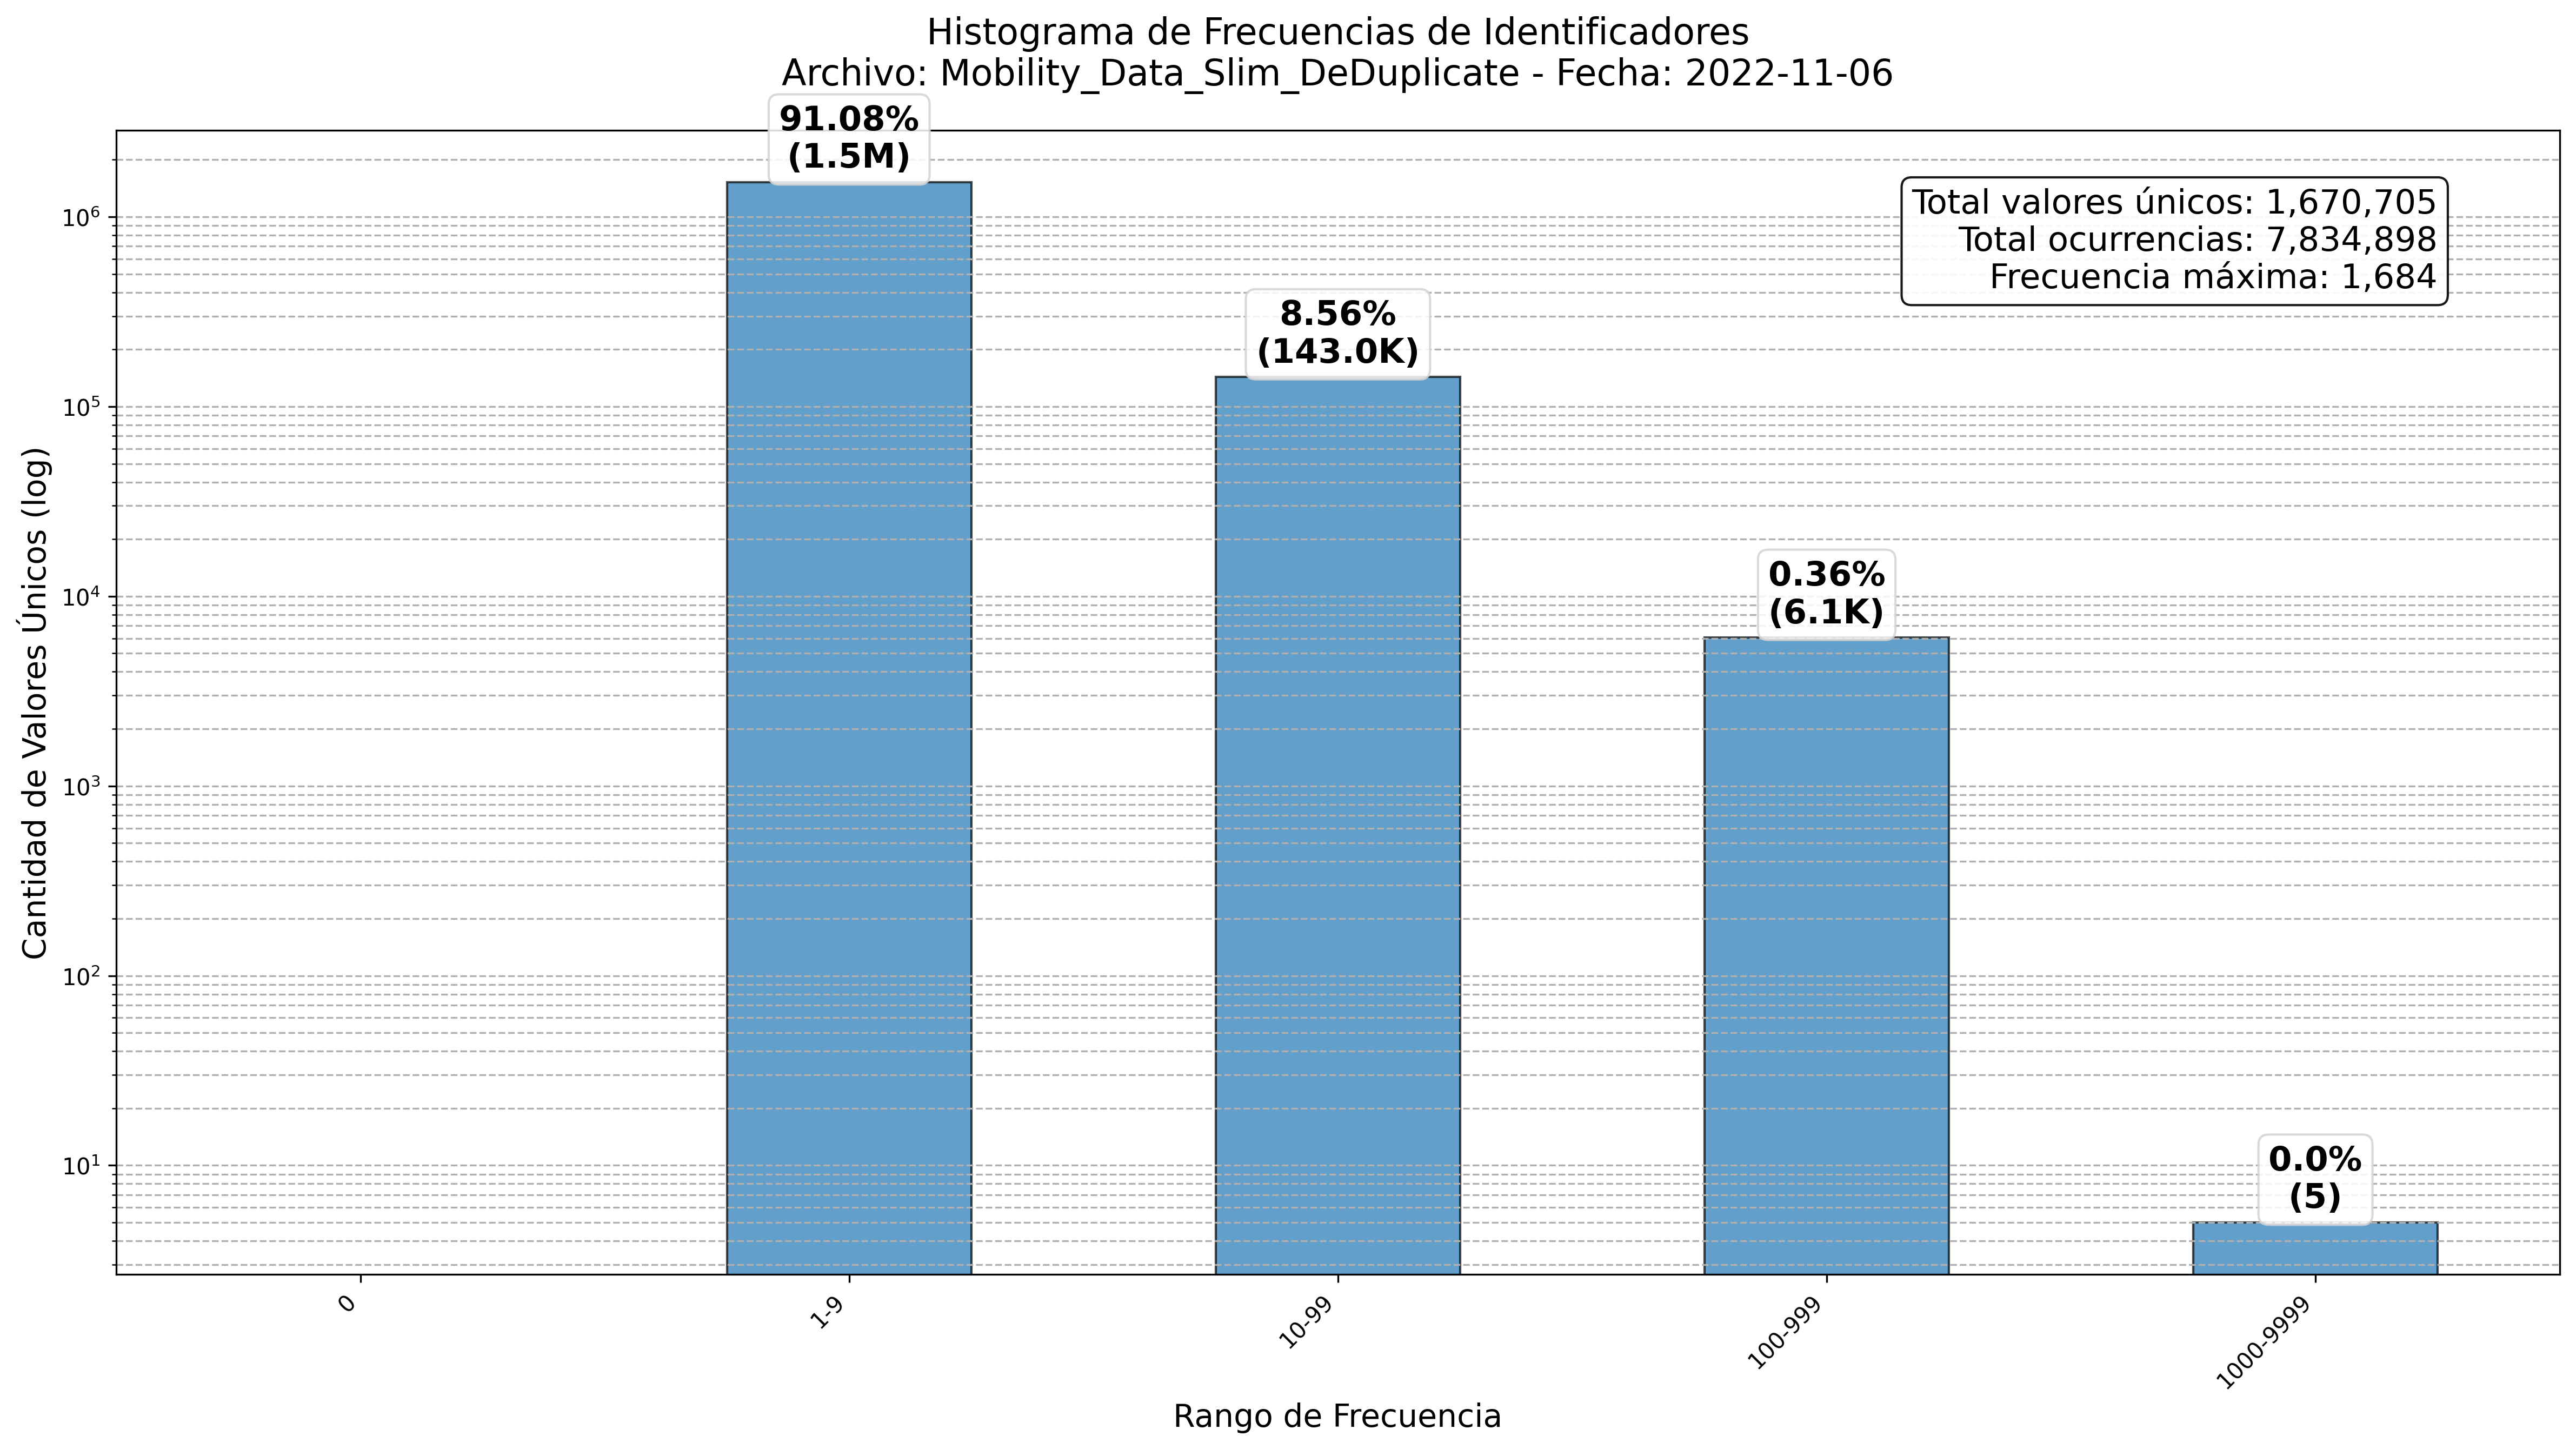
\includegraphics[width=\linewidth]{img/daily_histograms/histograma_identifier_Mobility_Data_Slim_DeDuplicate_2022-11-06.png}
        \caption{Histograma del 06/Nov/2022}
        \label{fig:sub1}
    \end{subfigure}
    \hfill
    \begin{subfigure}[t]{0.48\textwidth-1em}
        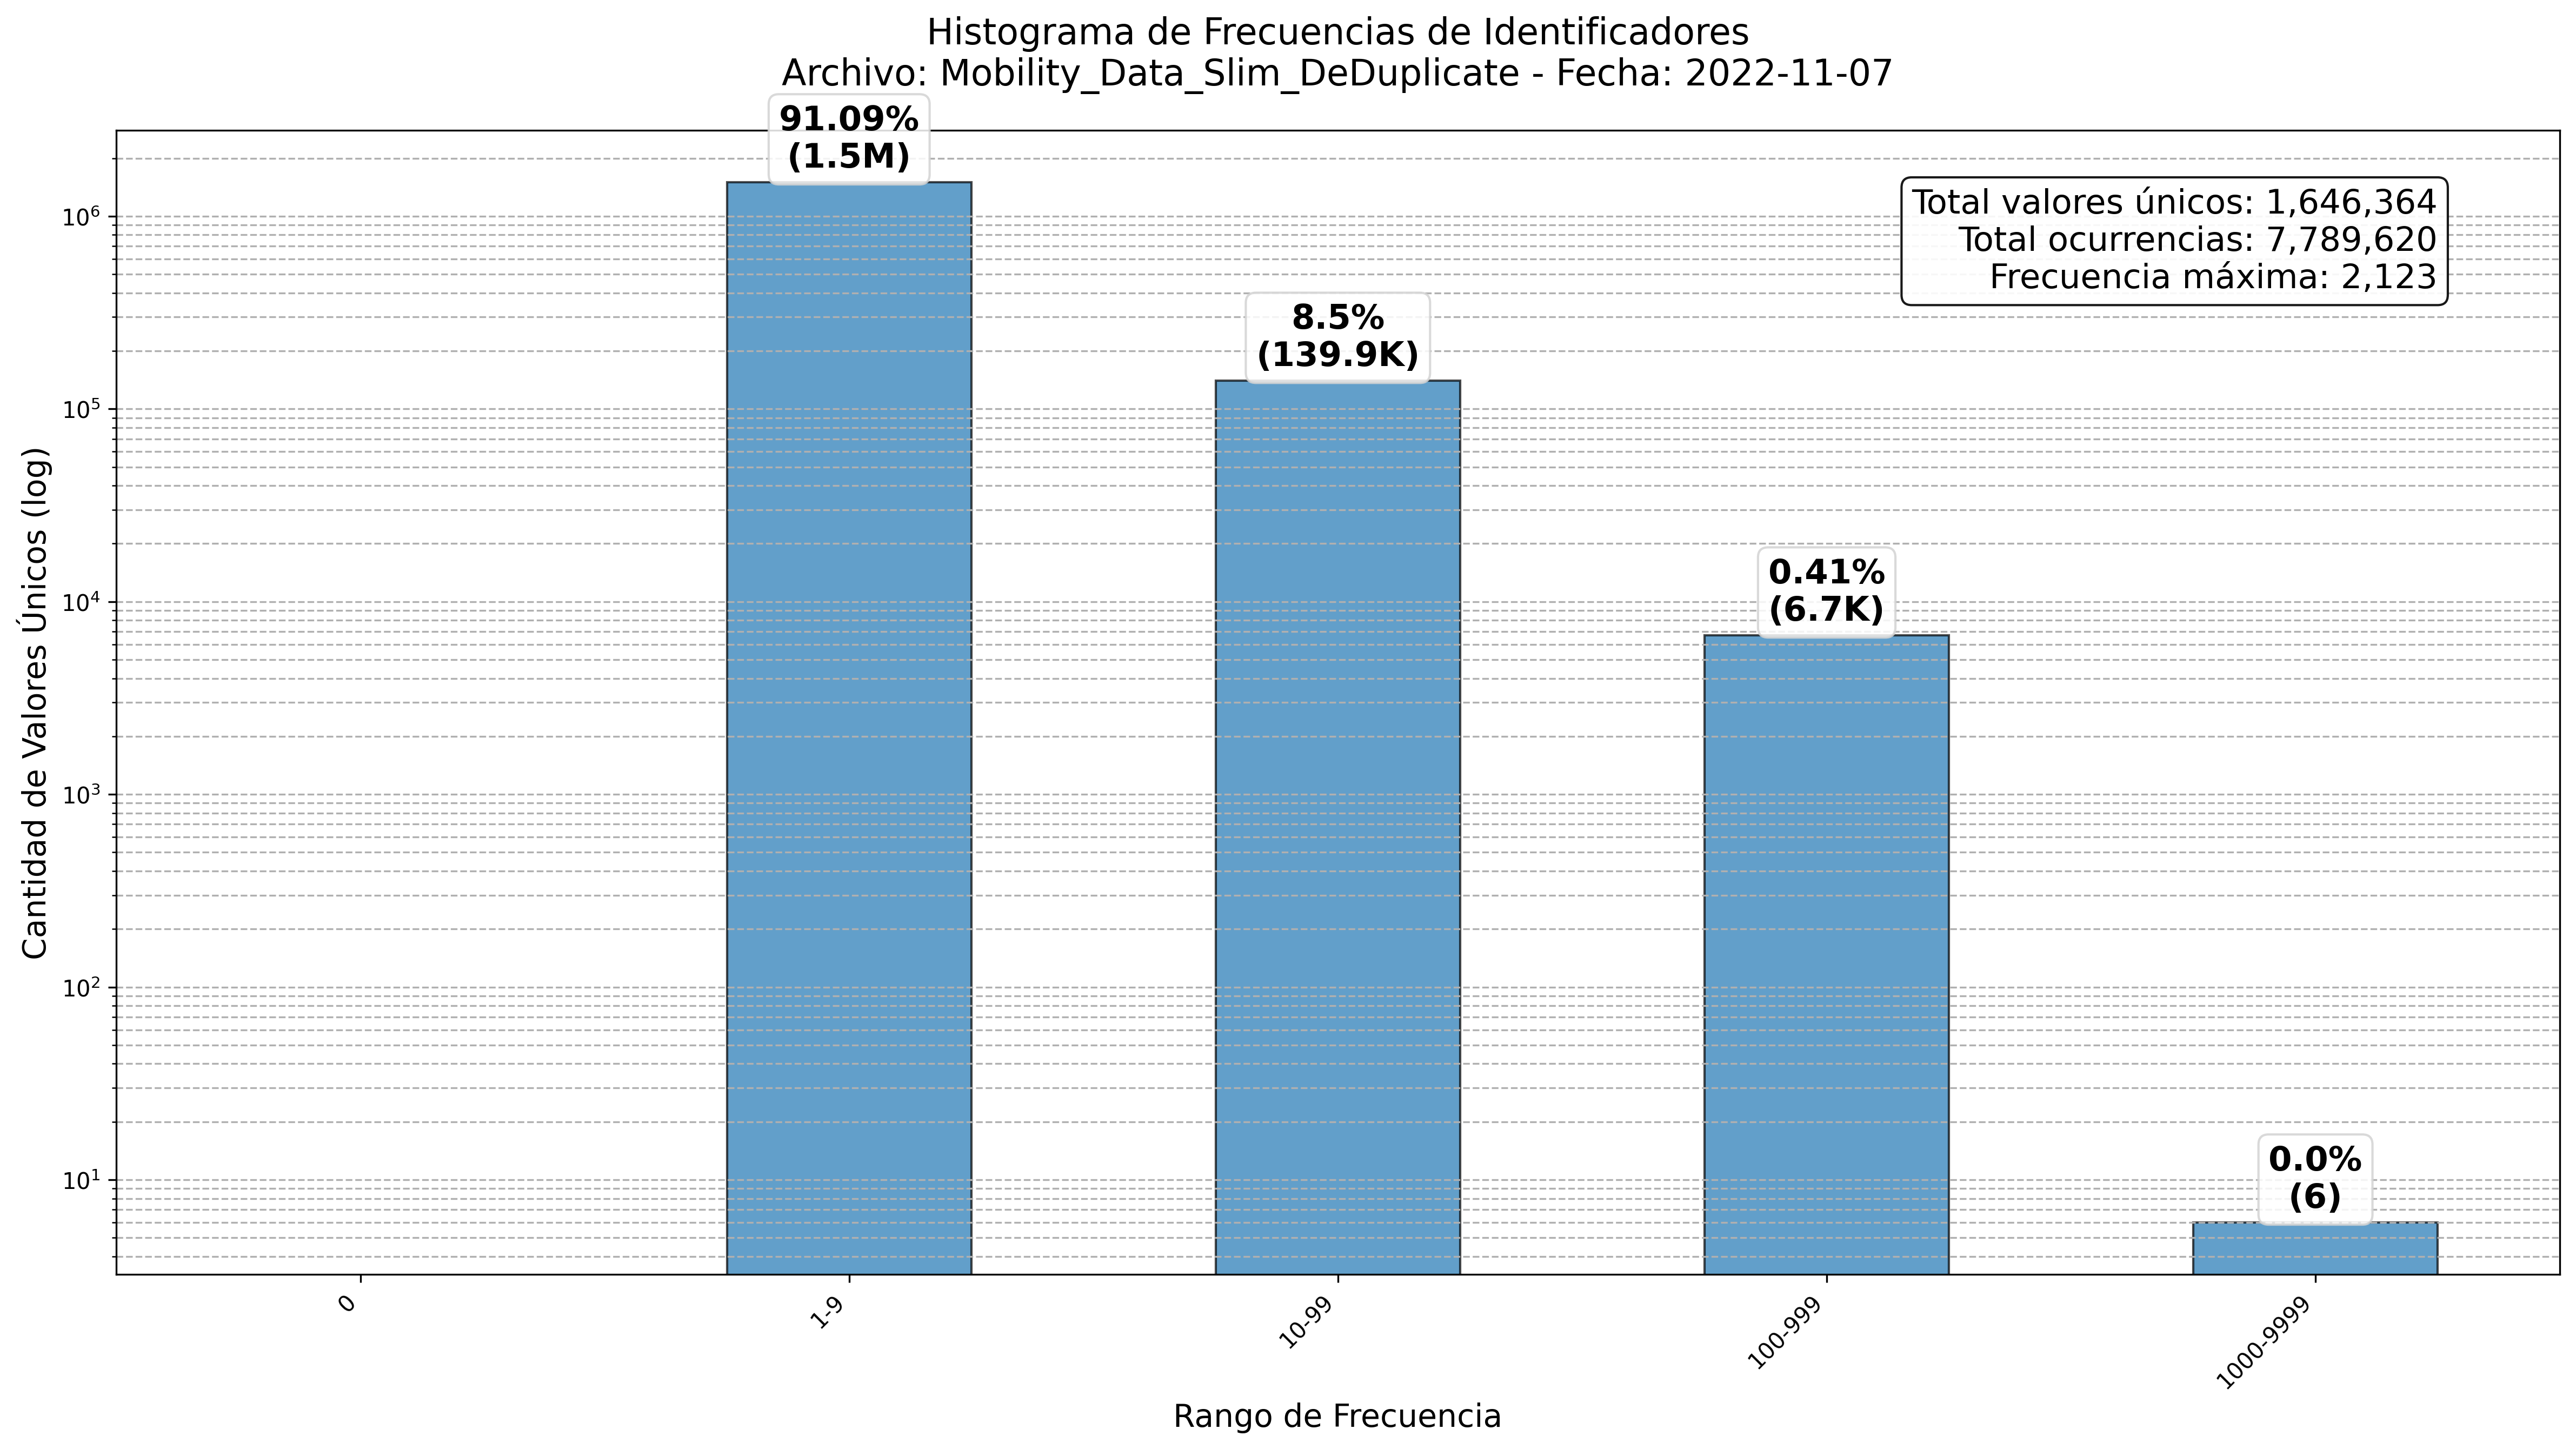
\includegraphics[width=\linewidth]{img/daily_histograms/histograma_identifier_Mobility_Data_Slim_DeDuplicate_2022-11-07.png}
        \caption{Histograma del 07/Nov/2022}
        \label{fig:sub2}
    \end{subfigure}

    \vspace{0.5cm}

    \begin{subfigure}[t]{0.48\textwidth-1em}
        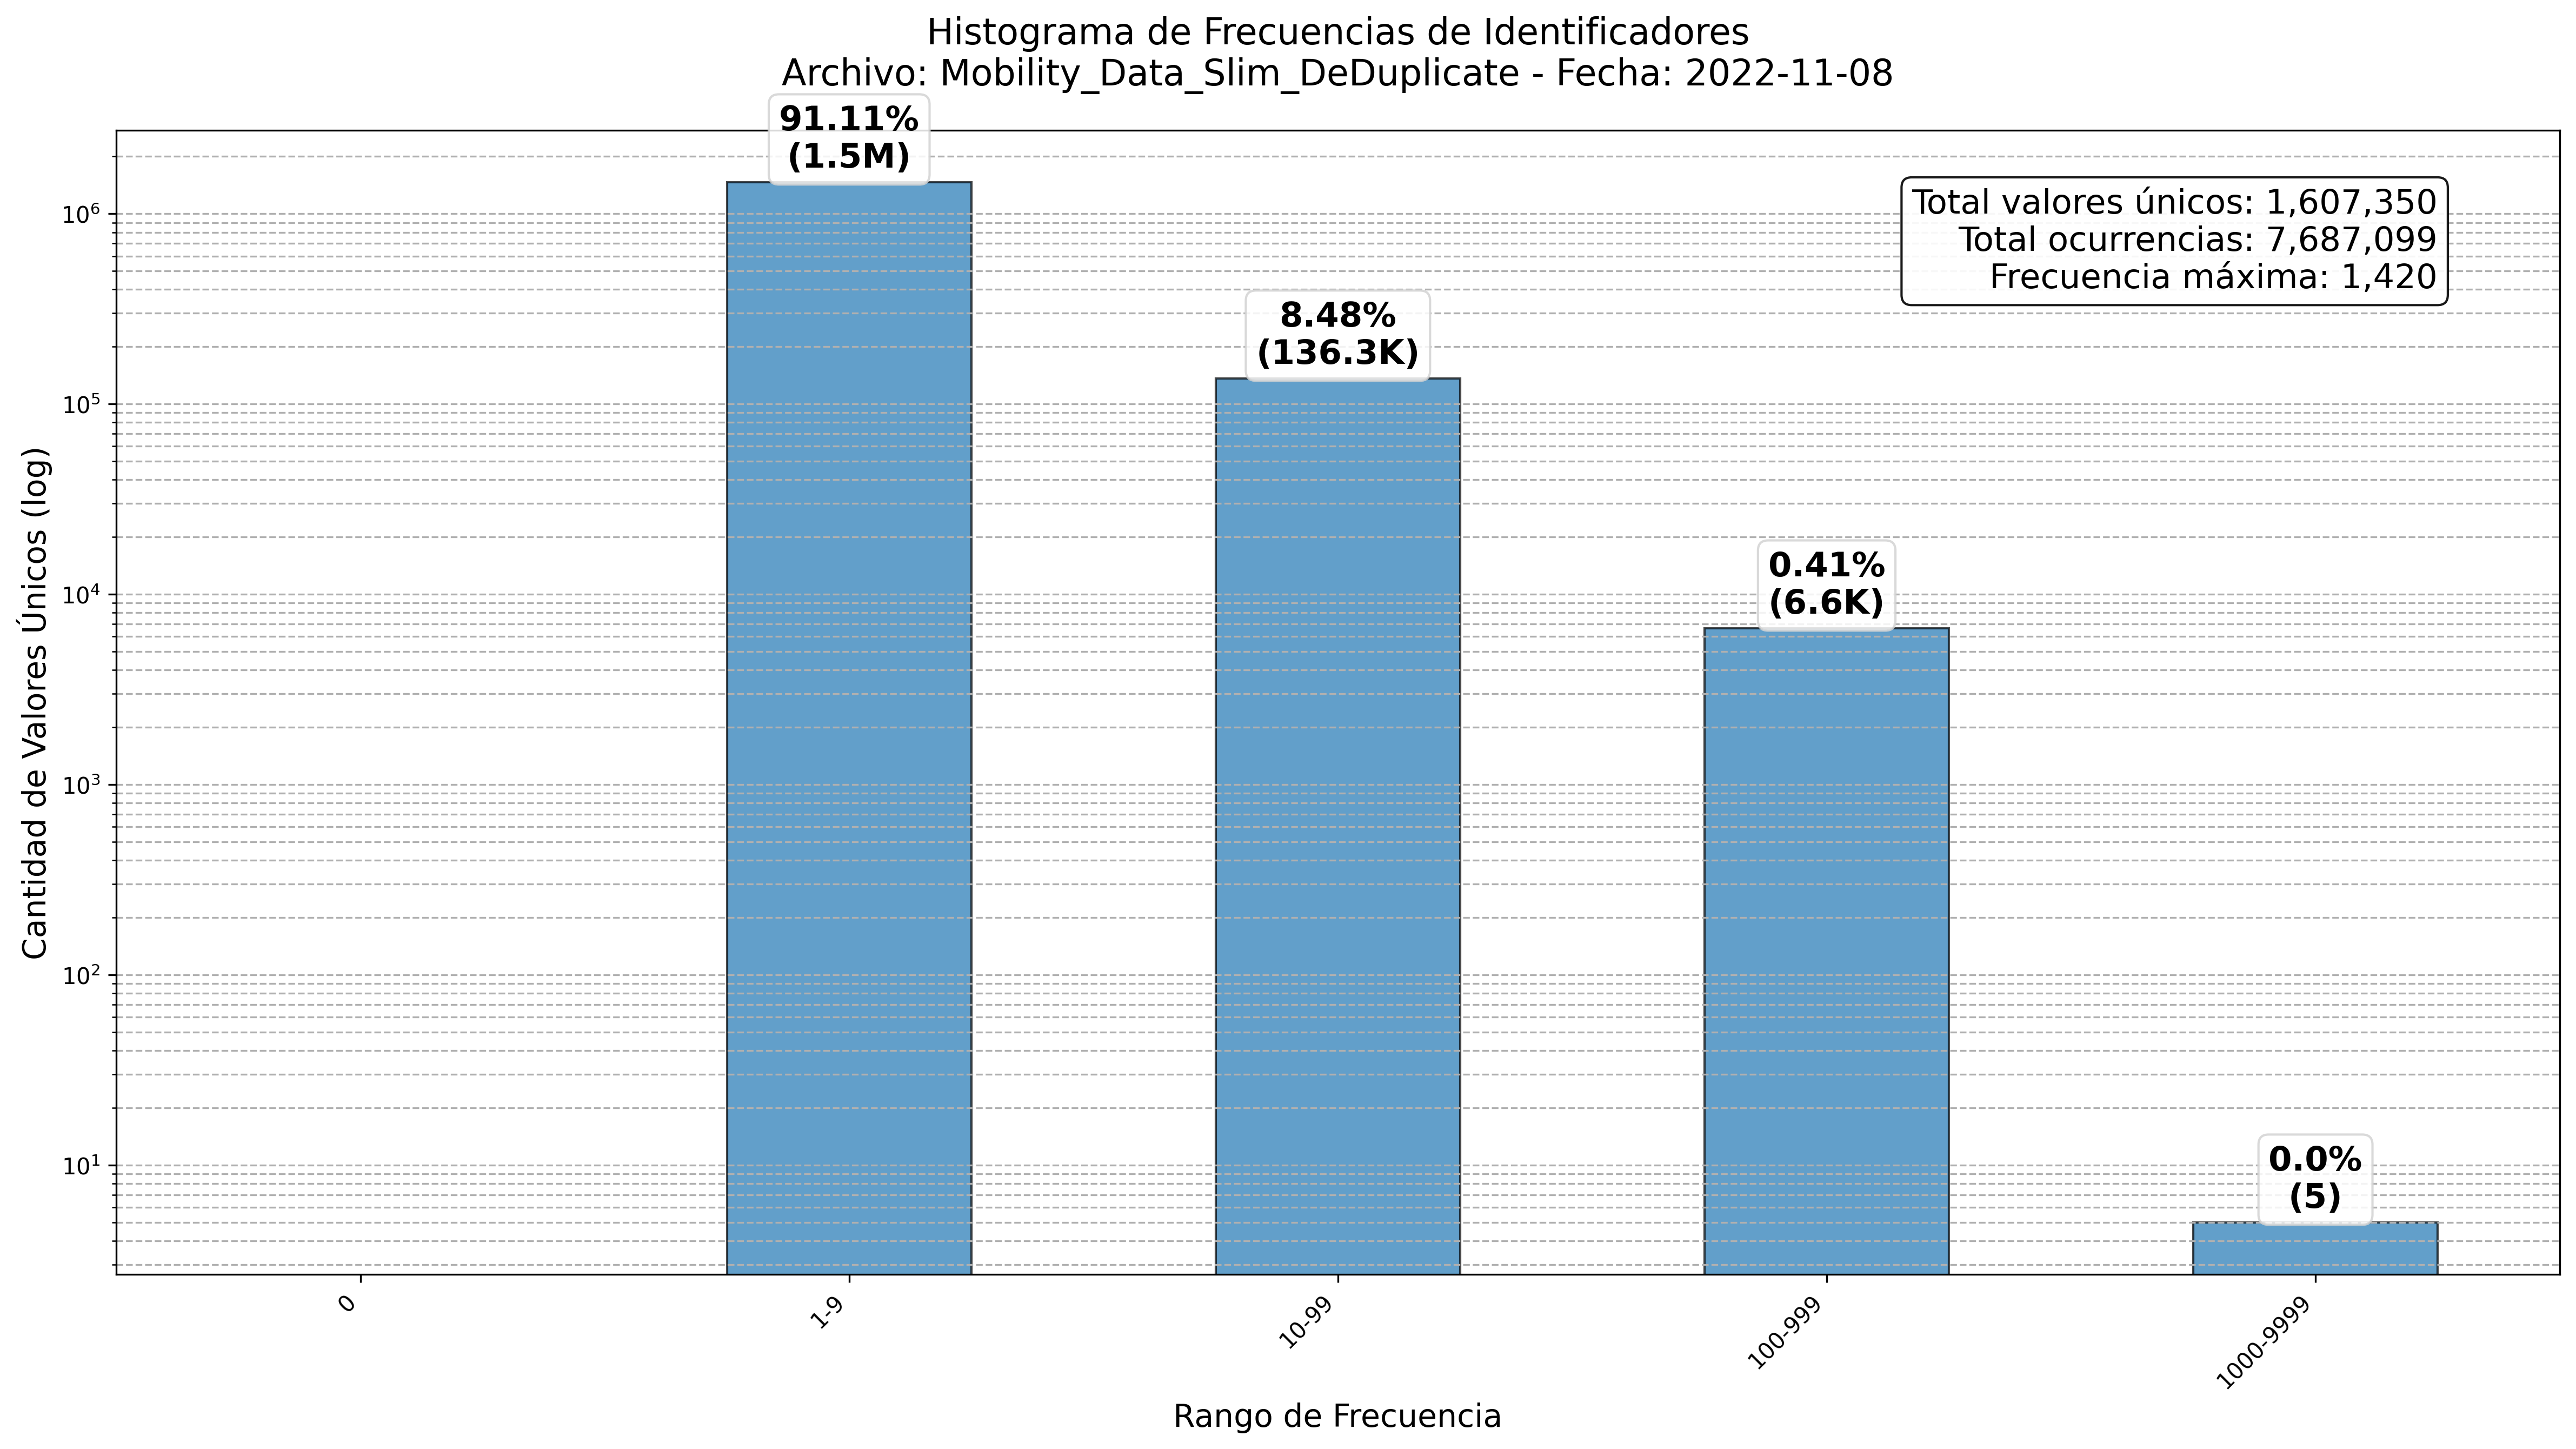
\includegraphics[width=\linewidth]{img/daily_histograms/histograma_identifier_Mobility_Data_Slim_DeDuplicate_2022-11-08.png}
        \caption{Histograma del 08/Nov/2022}
        \label{fig:sub3}
    \end{subfigure}
    \hfill
    \begin{subfigure}[t]{0.48\textwidth-1em}
        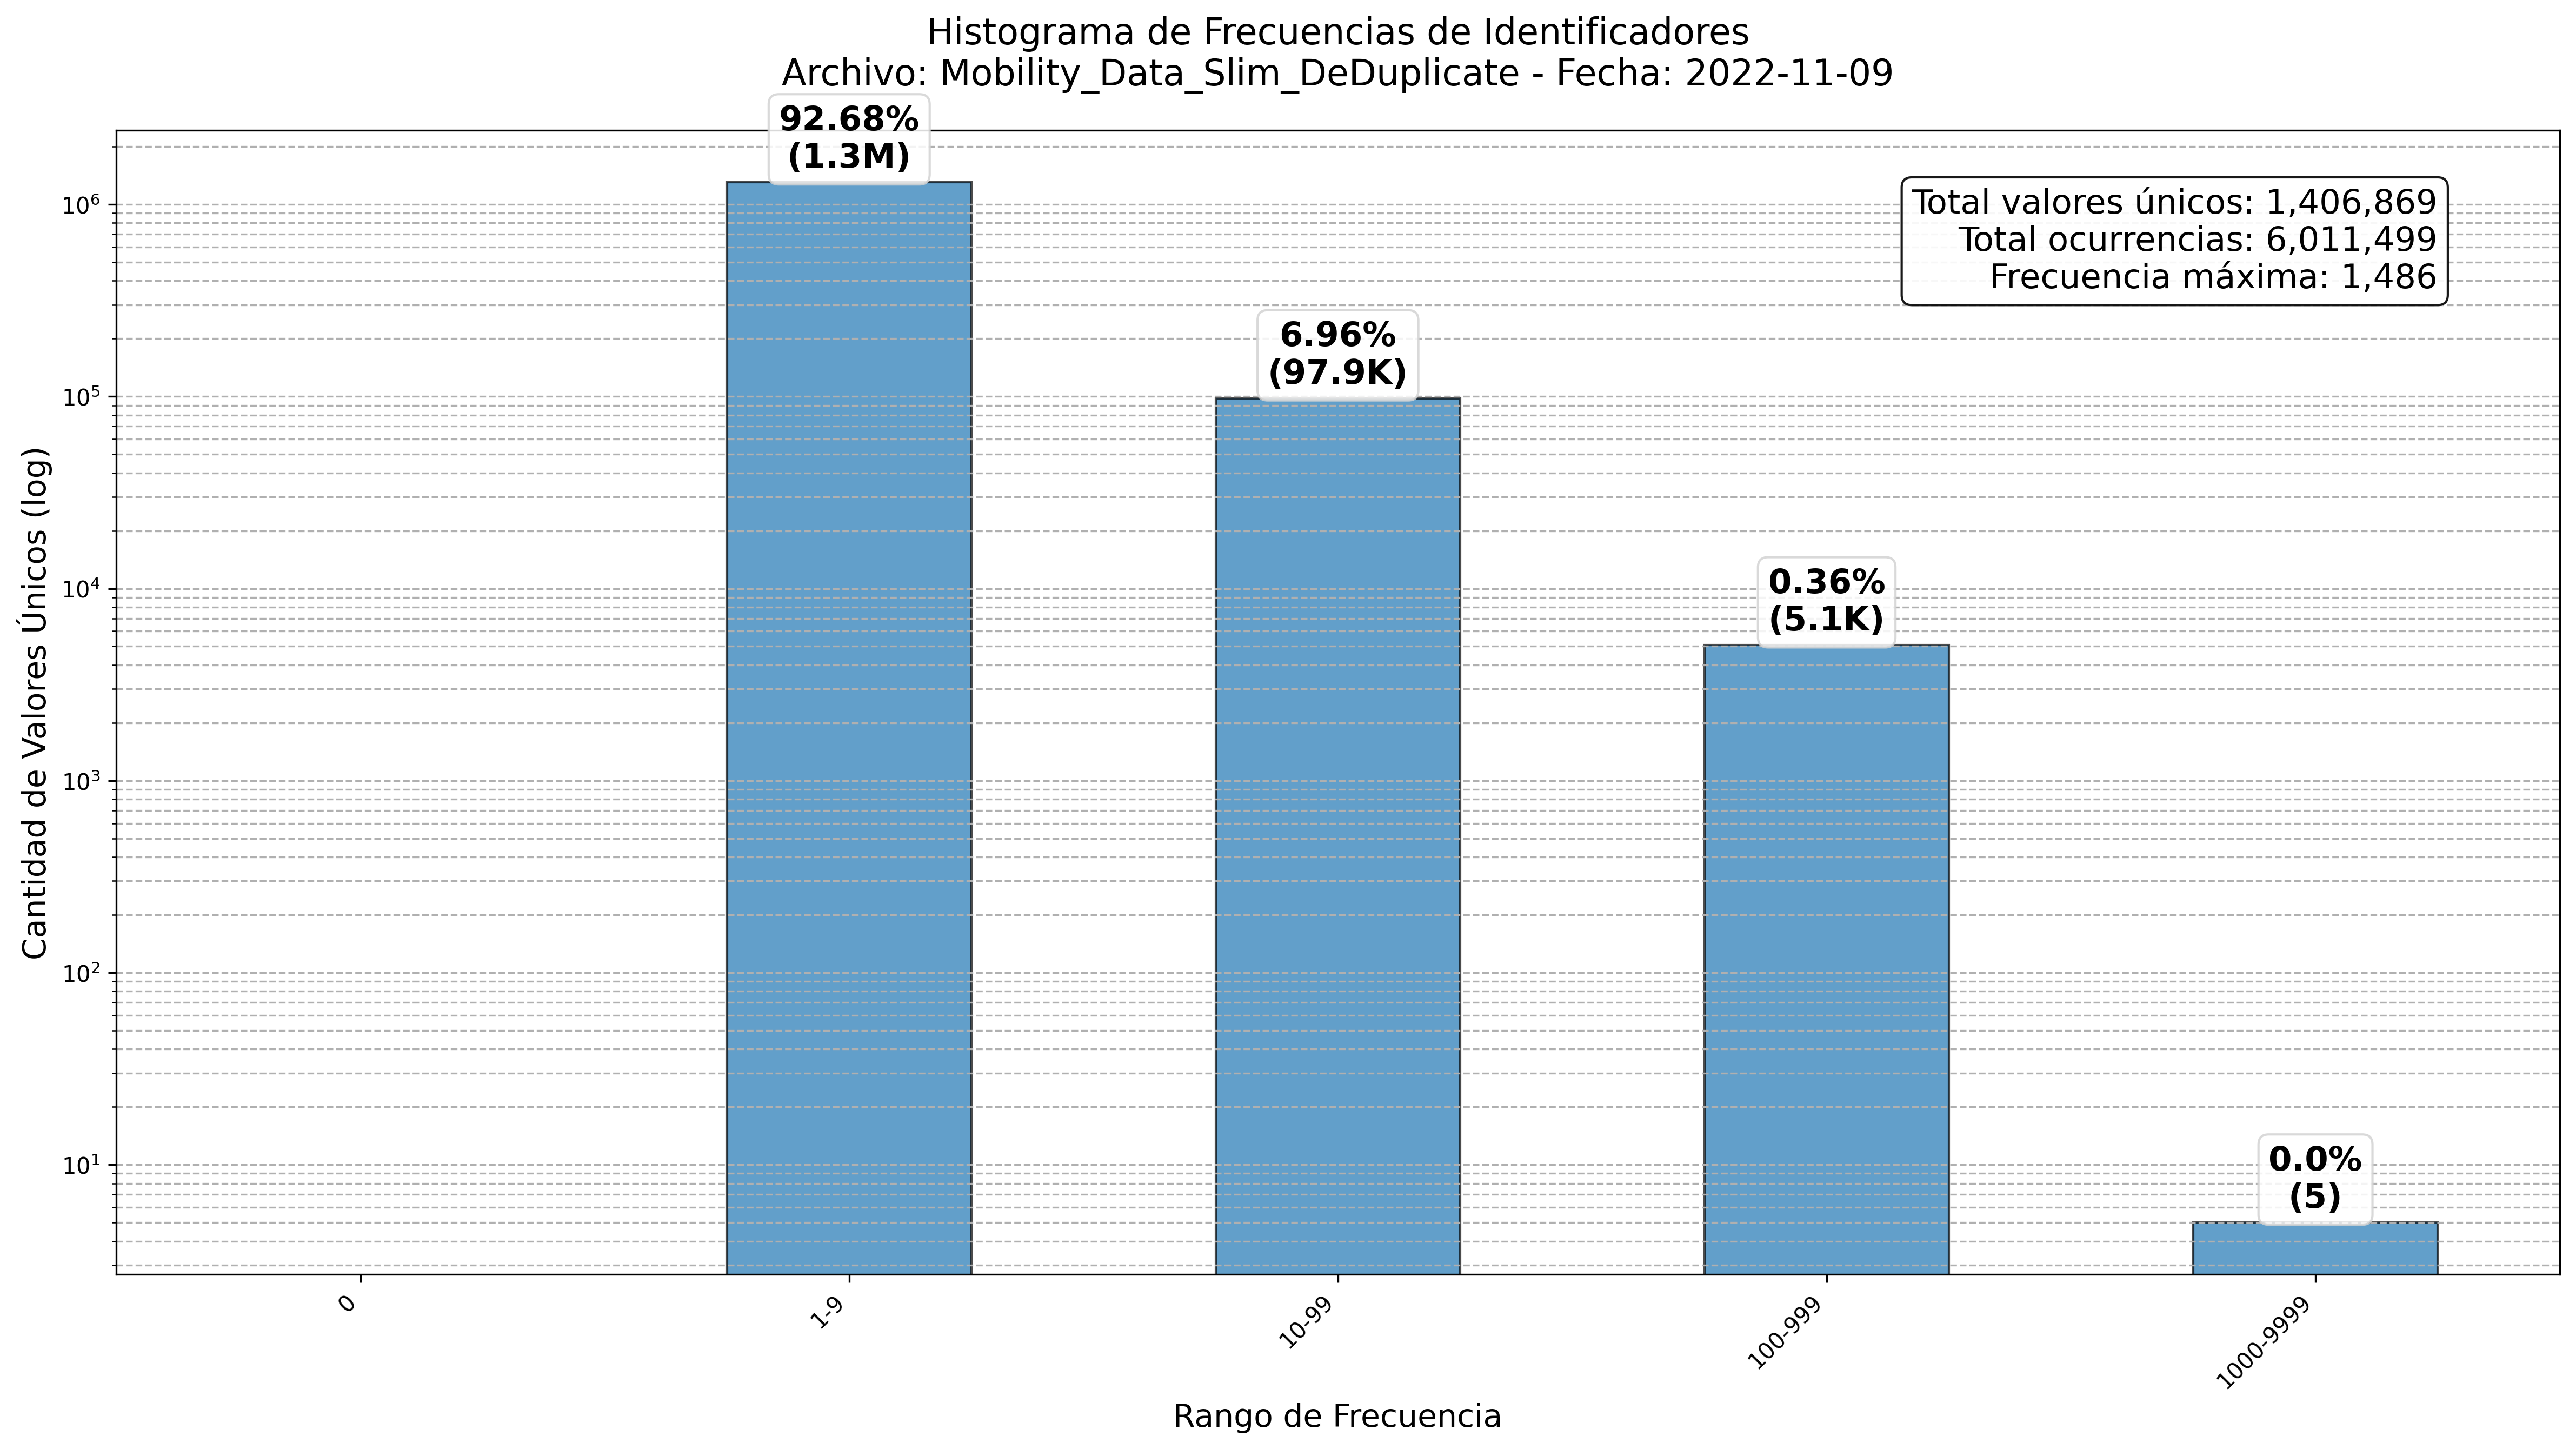
\includegraphics[width=\linewidth]{img/daily_histograms/histograma_identifier_Mobility_Data_Slim_DeDuplicate_2022-11-09.png}
        \caption{Histograma del 09/Nov/2022}
        \label{fig:sub4}
    \end{subfigure}
\end{figure}

\begin{figure}[H]
    \ContinuedFloat
    \centering
    \begin{subfigure}[t]{0.48\textwidth-1em}
        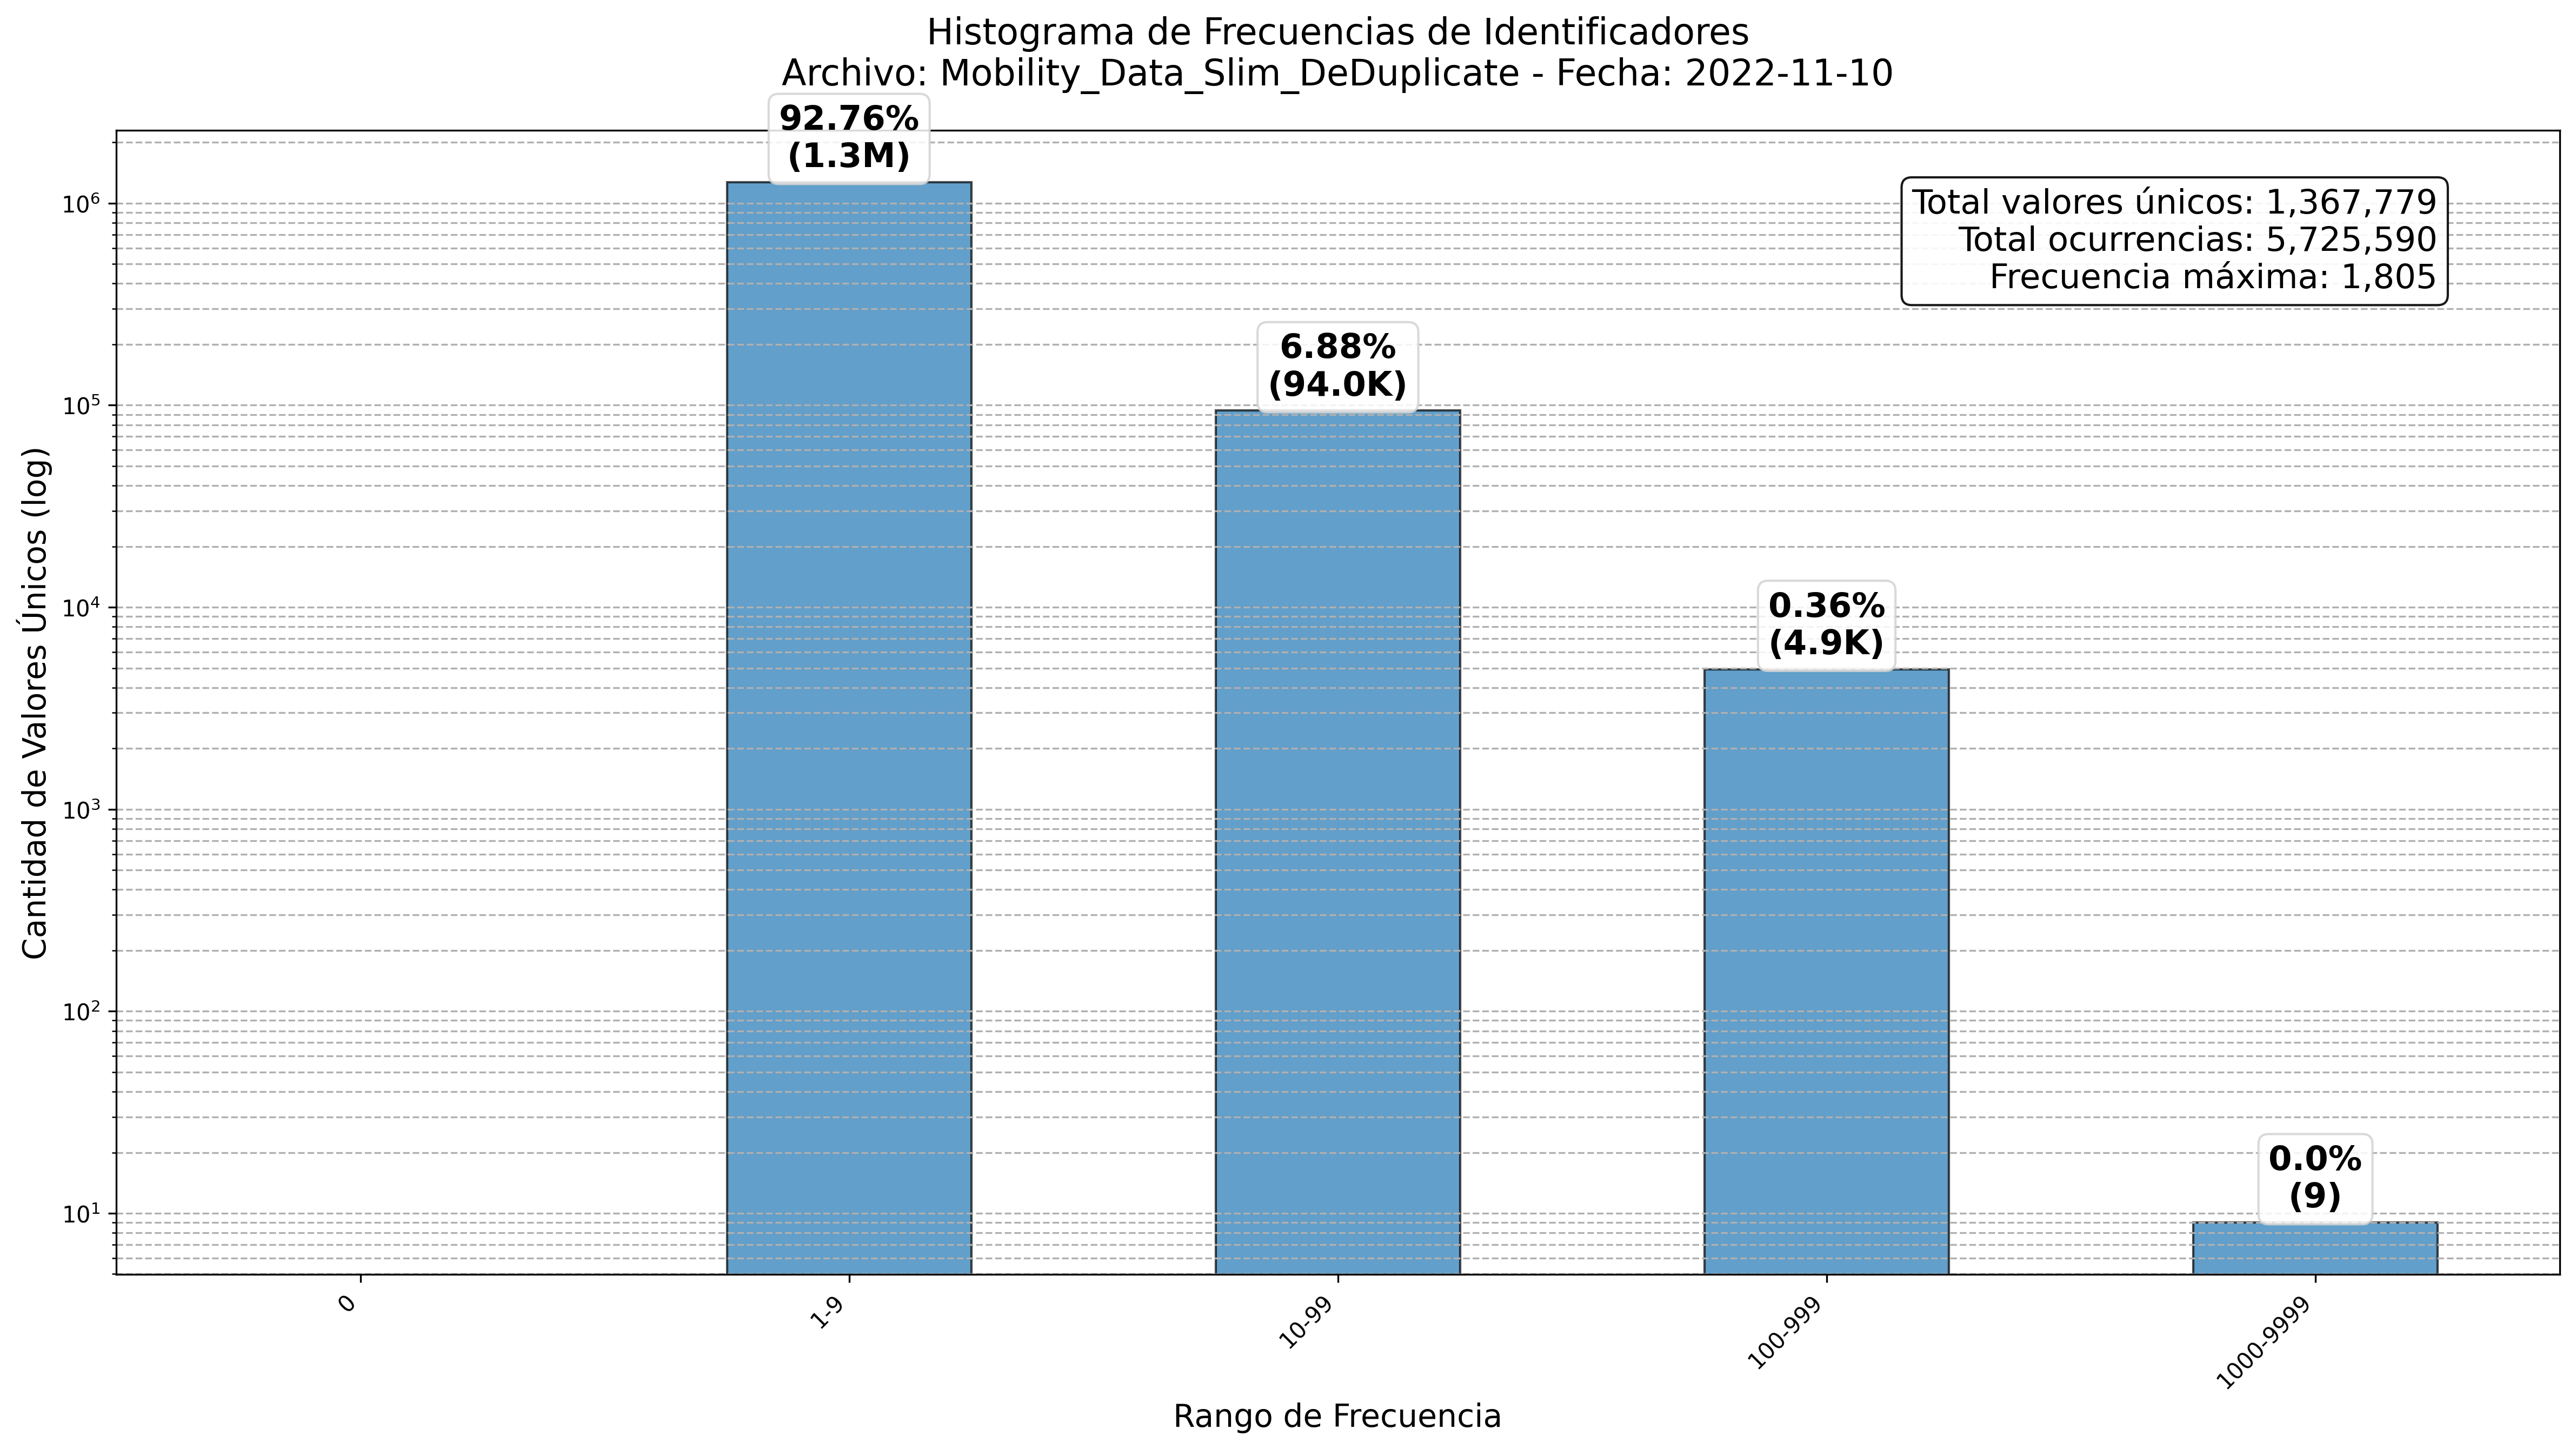
\includegraphics[width=\linewidth]{img/daily_histograms/histograma_identifier_Mobility_Data_Slim_DeDuplicate_2022-11-10.png}
        \caption{Histograma del 10/Nov/2022}
        \label{fig:sub5}
    \end{subfigure}
    \hfill
    \begin{subfigure}[t]{0.48\textwidth-1em}
        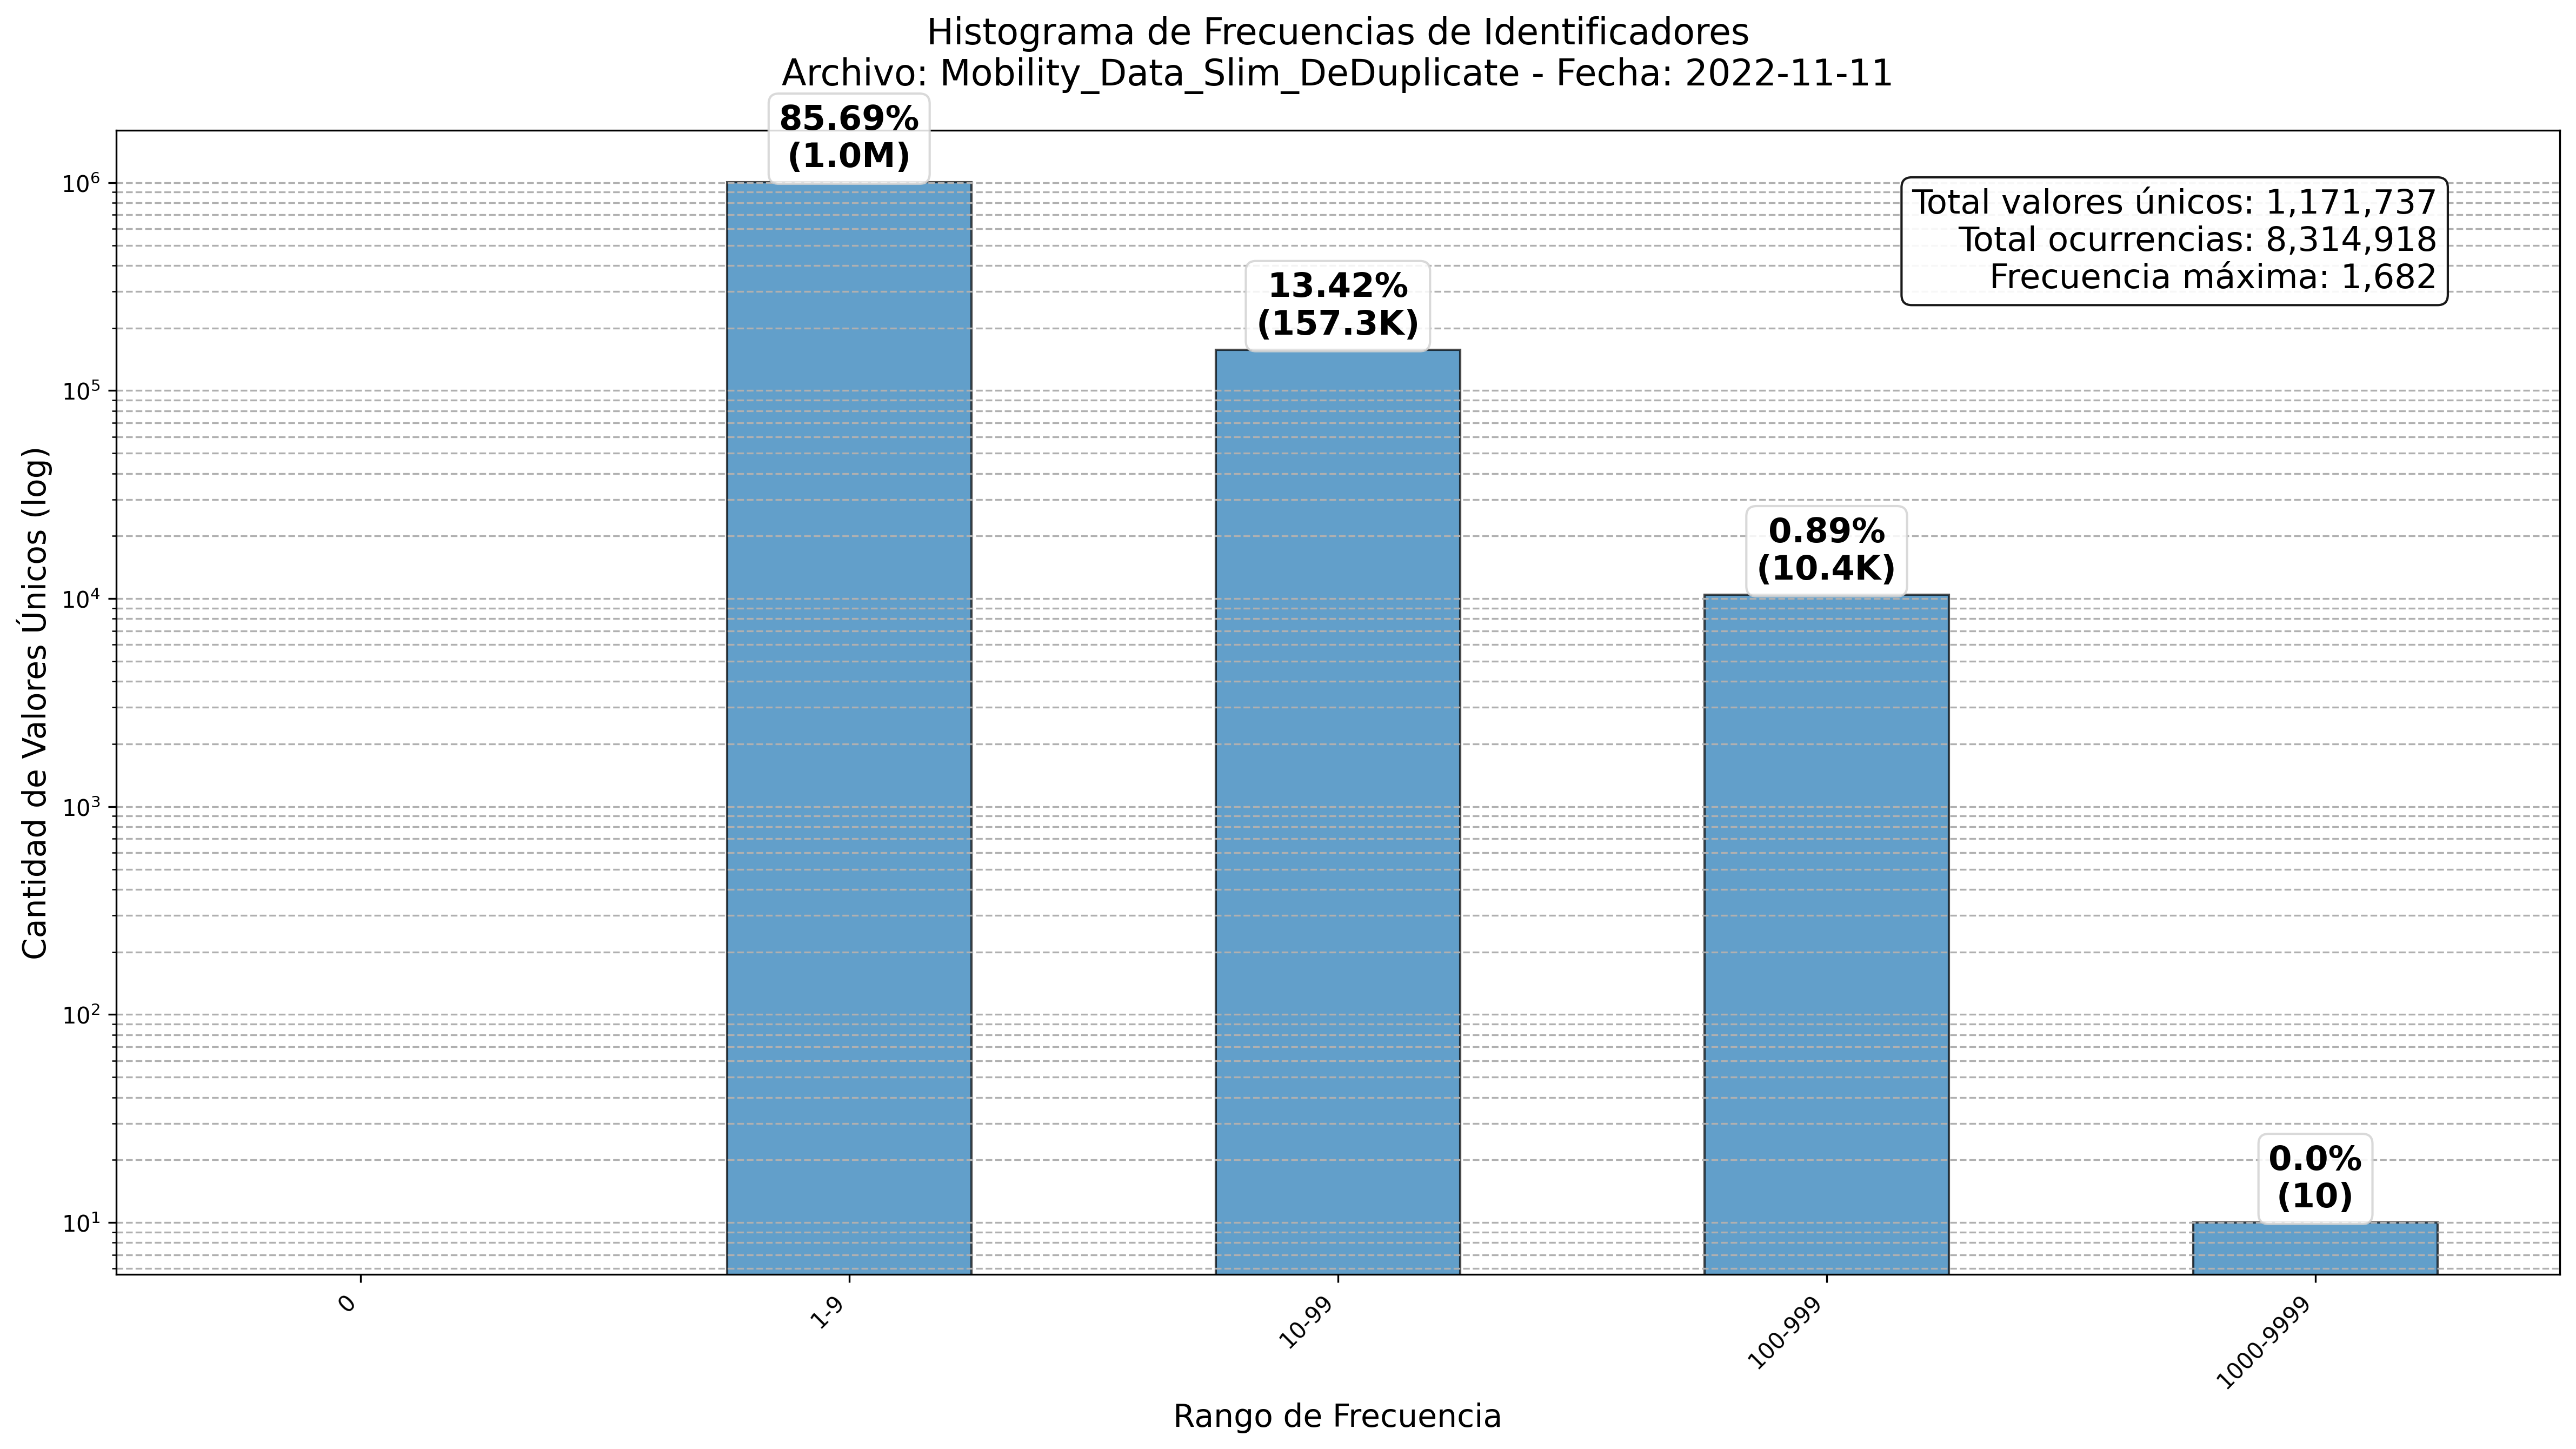
\includegraphics[width=\linewidth]{img/daily_histograms/histograma_identifier_Mobility_Data_Slim_DeDuplicate_2022-11-11.png}
        \caption{Histograma del 11/Nov/2022}
        \label{fig:sub6}
    \end{subfigure}

    \vspace{0.5cm}

    \begin{subfigure}[t]{0.48\textwidth-1em}
        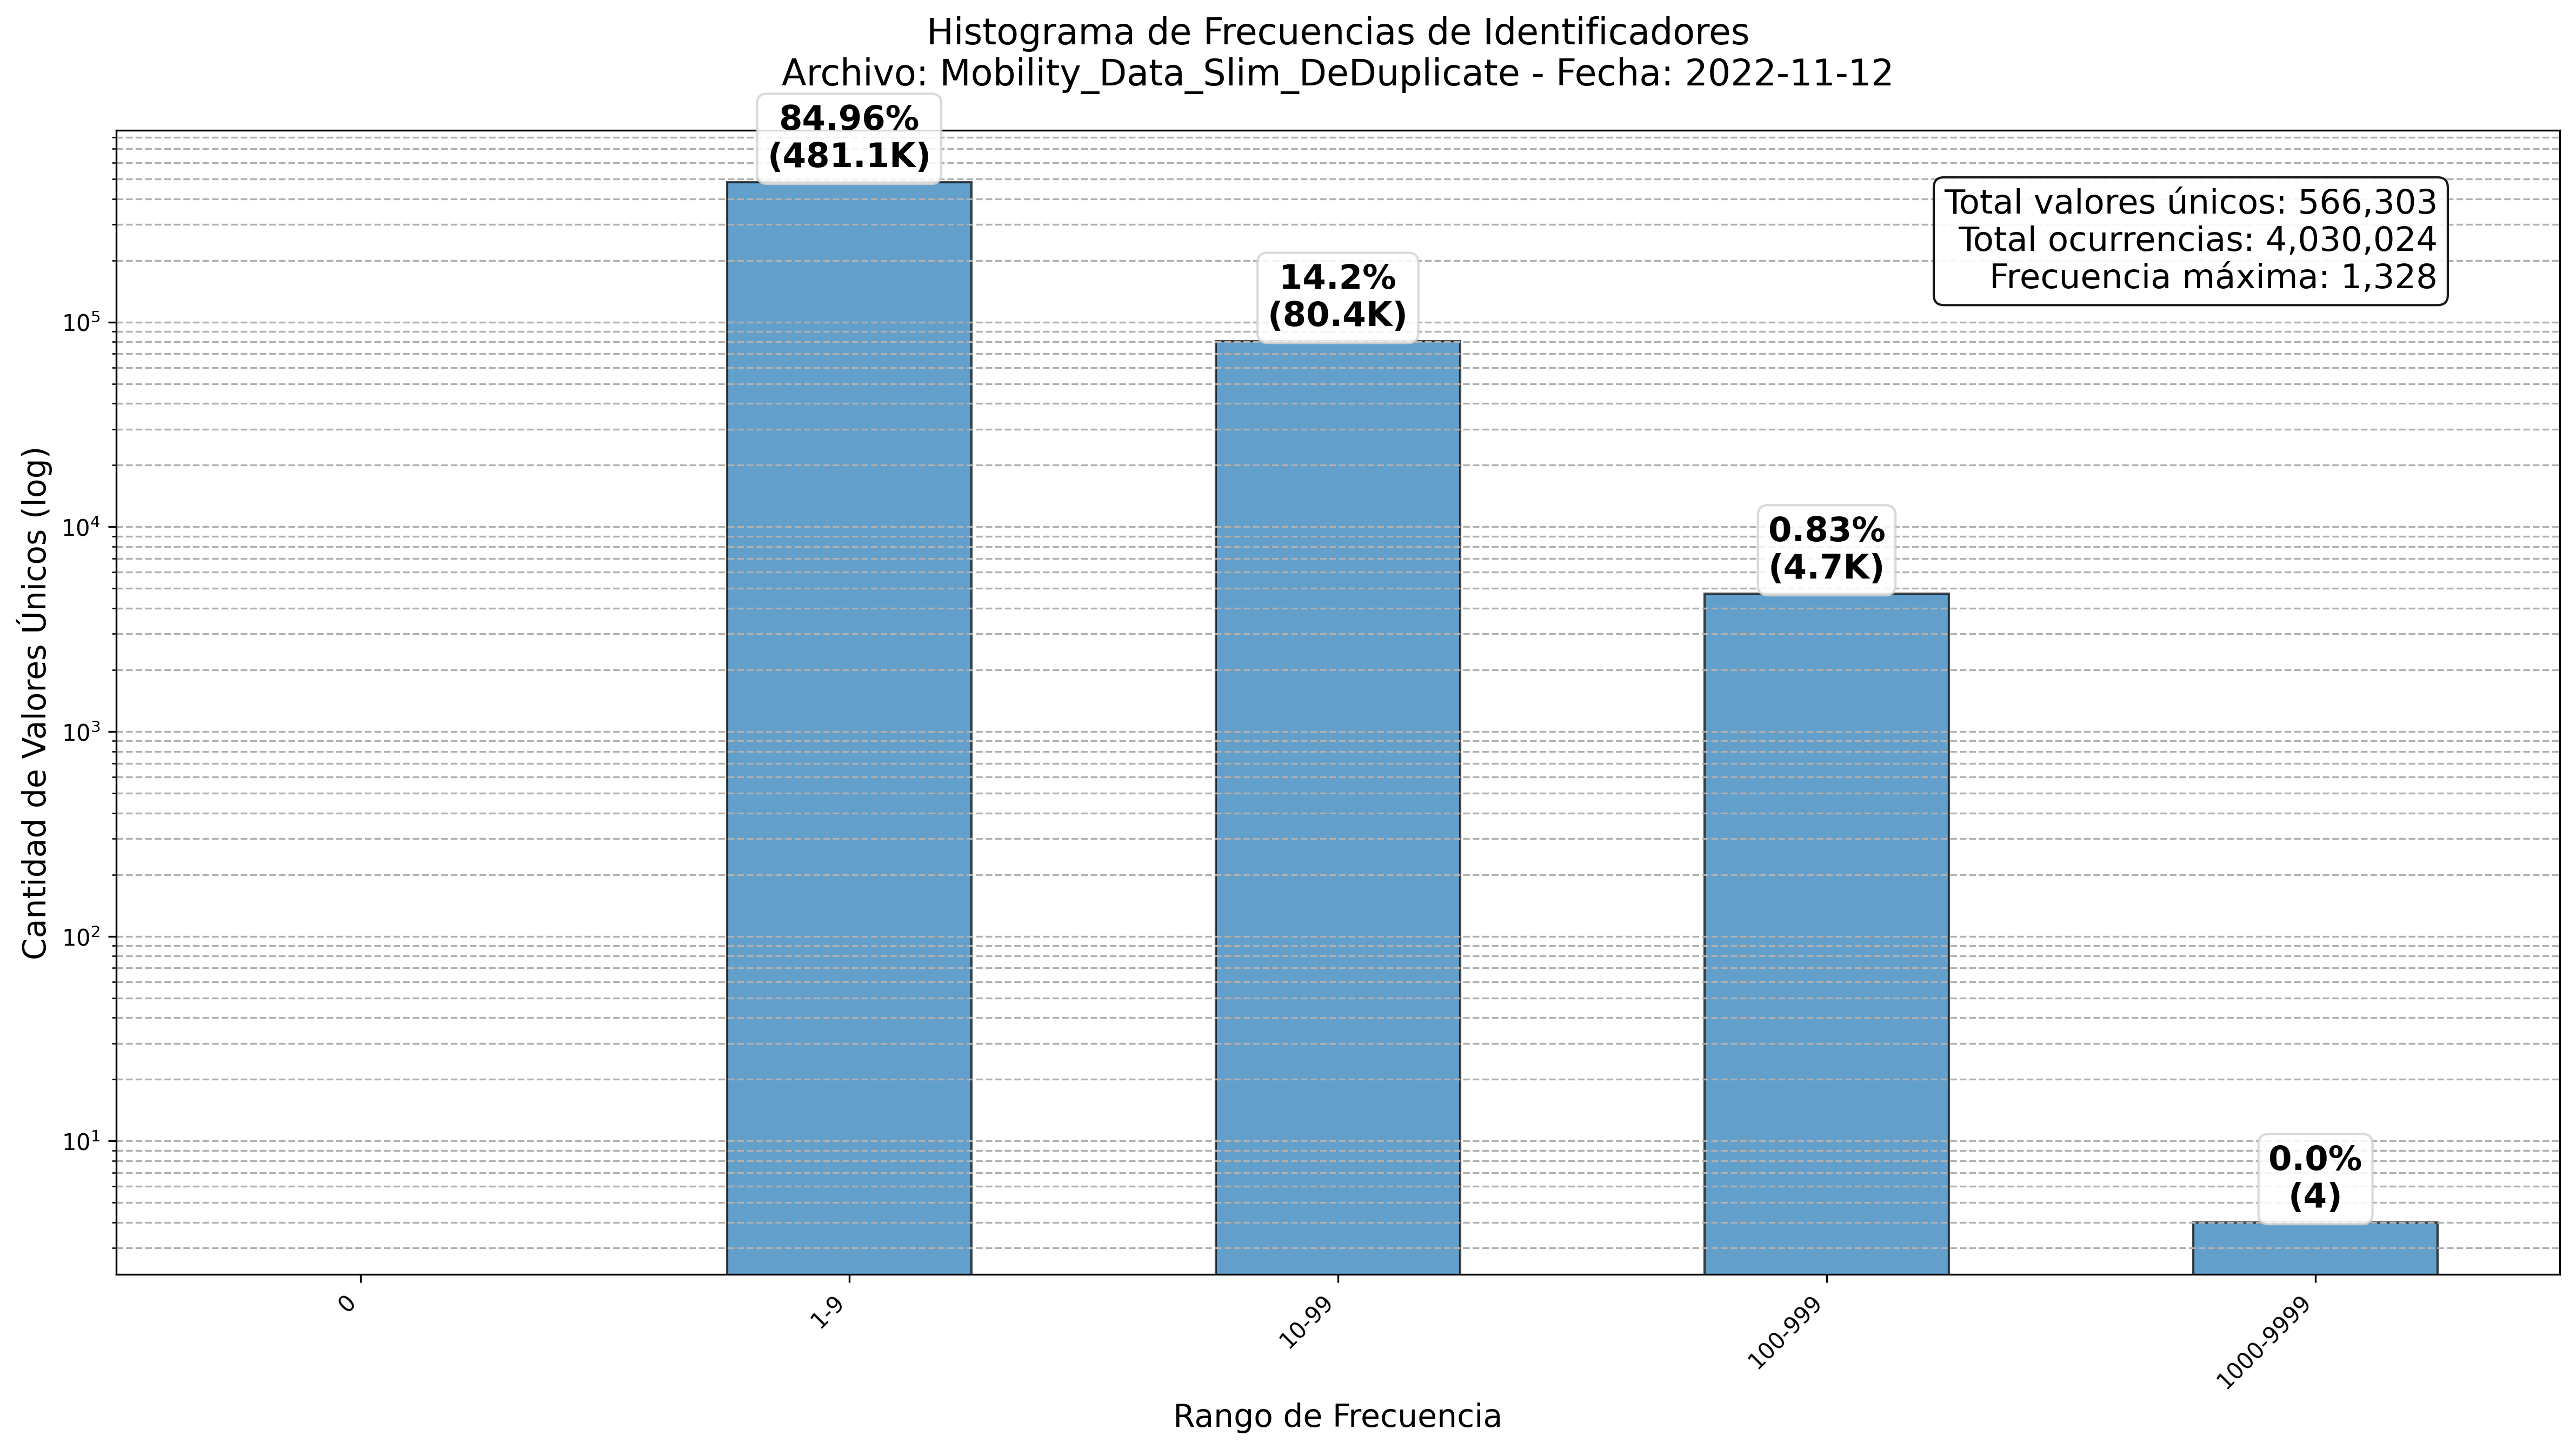
\includegraphics[width=\linewidth]{img/daily_histograms/histograma_identifier_Mobility_Data_Slim_DeDuplicate_2022-11-12.png}
        \caption{Histograma del 12/Nov/2022}
        \label{fig:sub7}
    \end{subfigure}
    \hfill
    \begin{subfigure}[t]{0.48\textwidth-1em}
        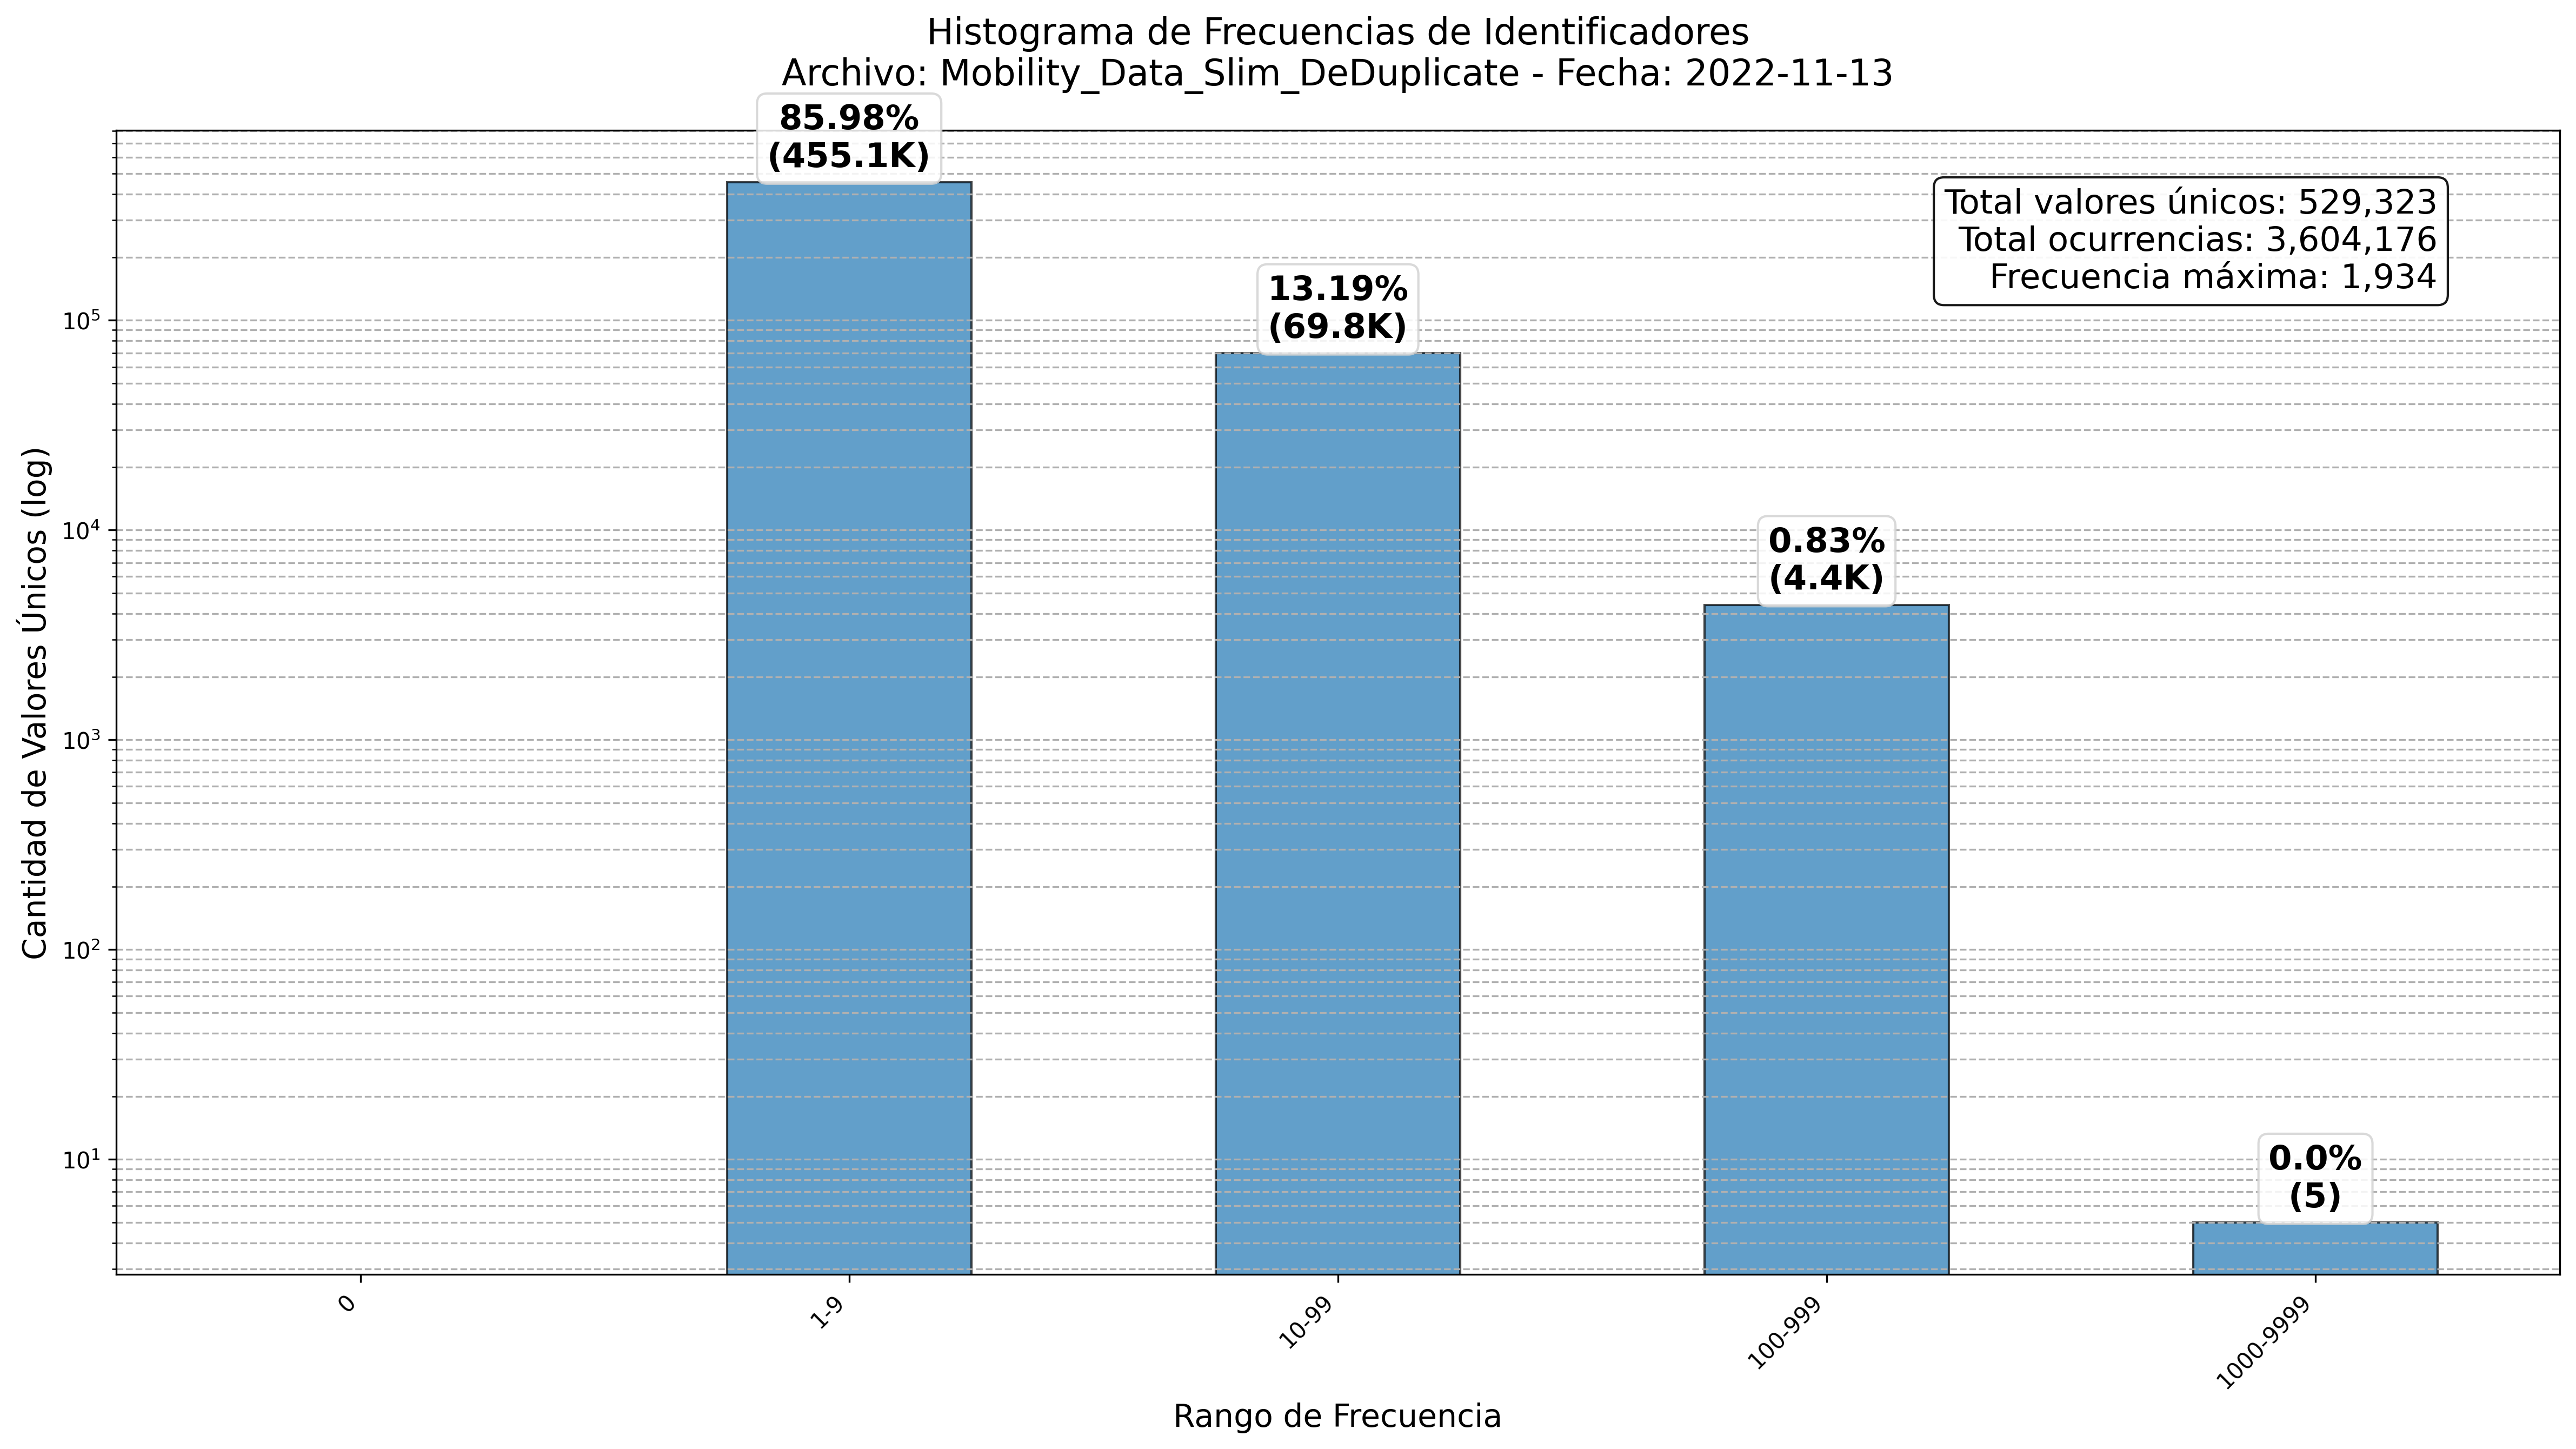
\includegraphics[width=\linewidth]{img/daily_histograms/histograma_identifier_Mobility_Data_Slim_DeDuplicate_2022-11-13.png}
        \caption{Histograma del 13/Nov/2022}
        \label{fig:sub8}
    \end{subfigure}

    \vspace{0.5cm}

    \begin{subfigure}[t]{0.48\textwidth-1em}
        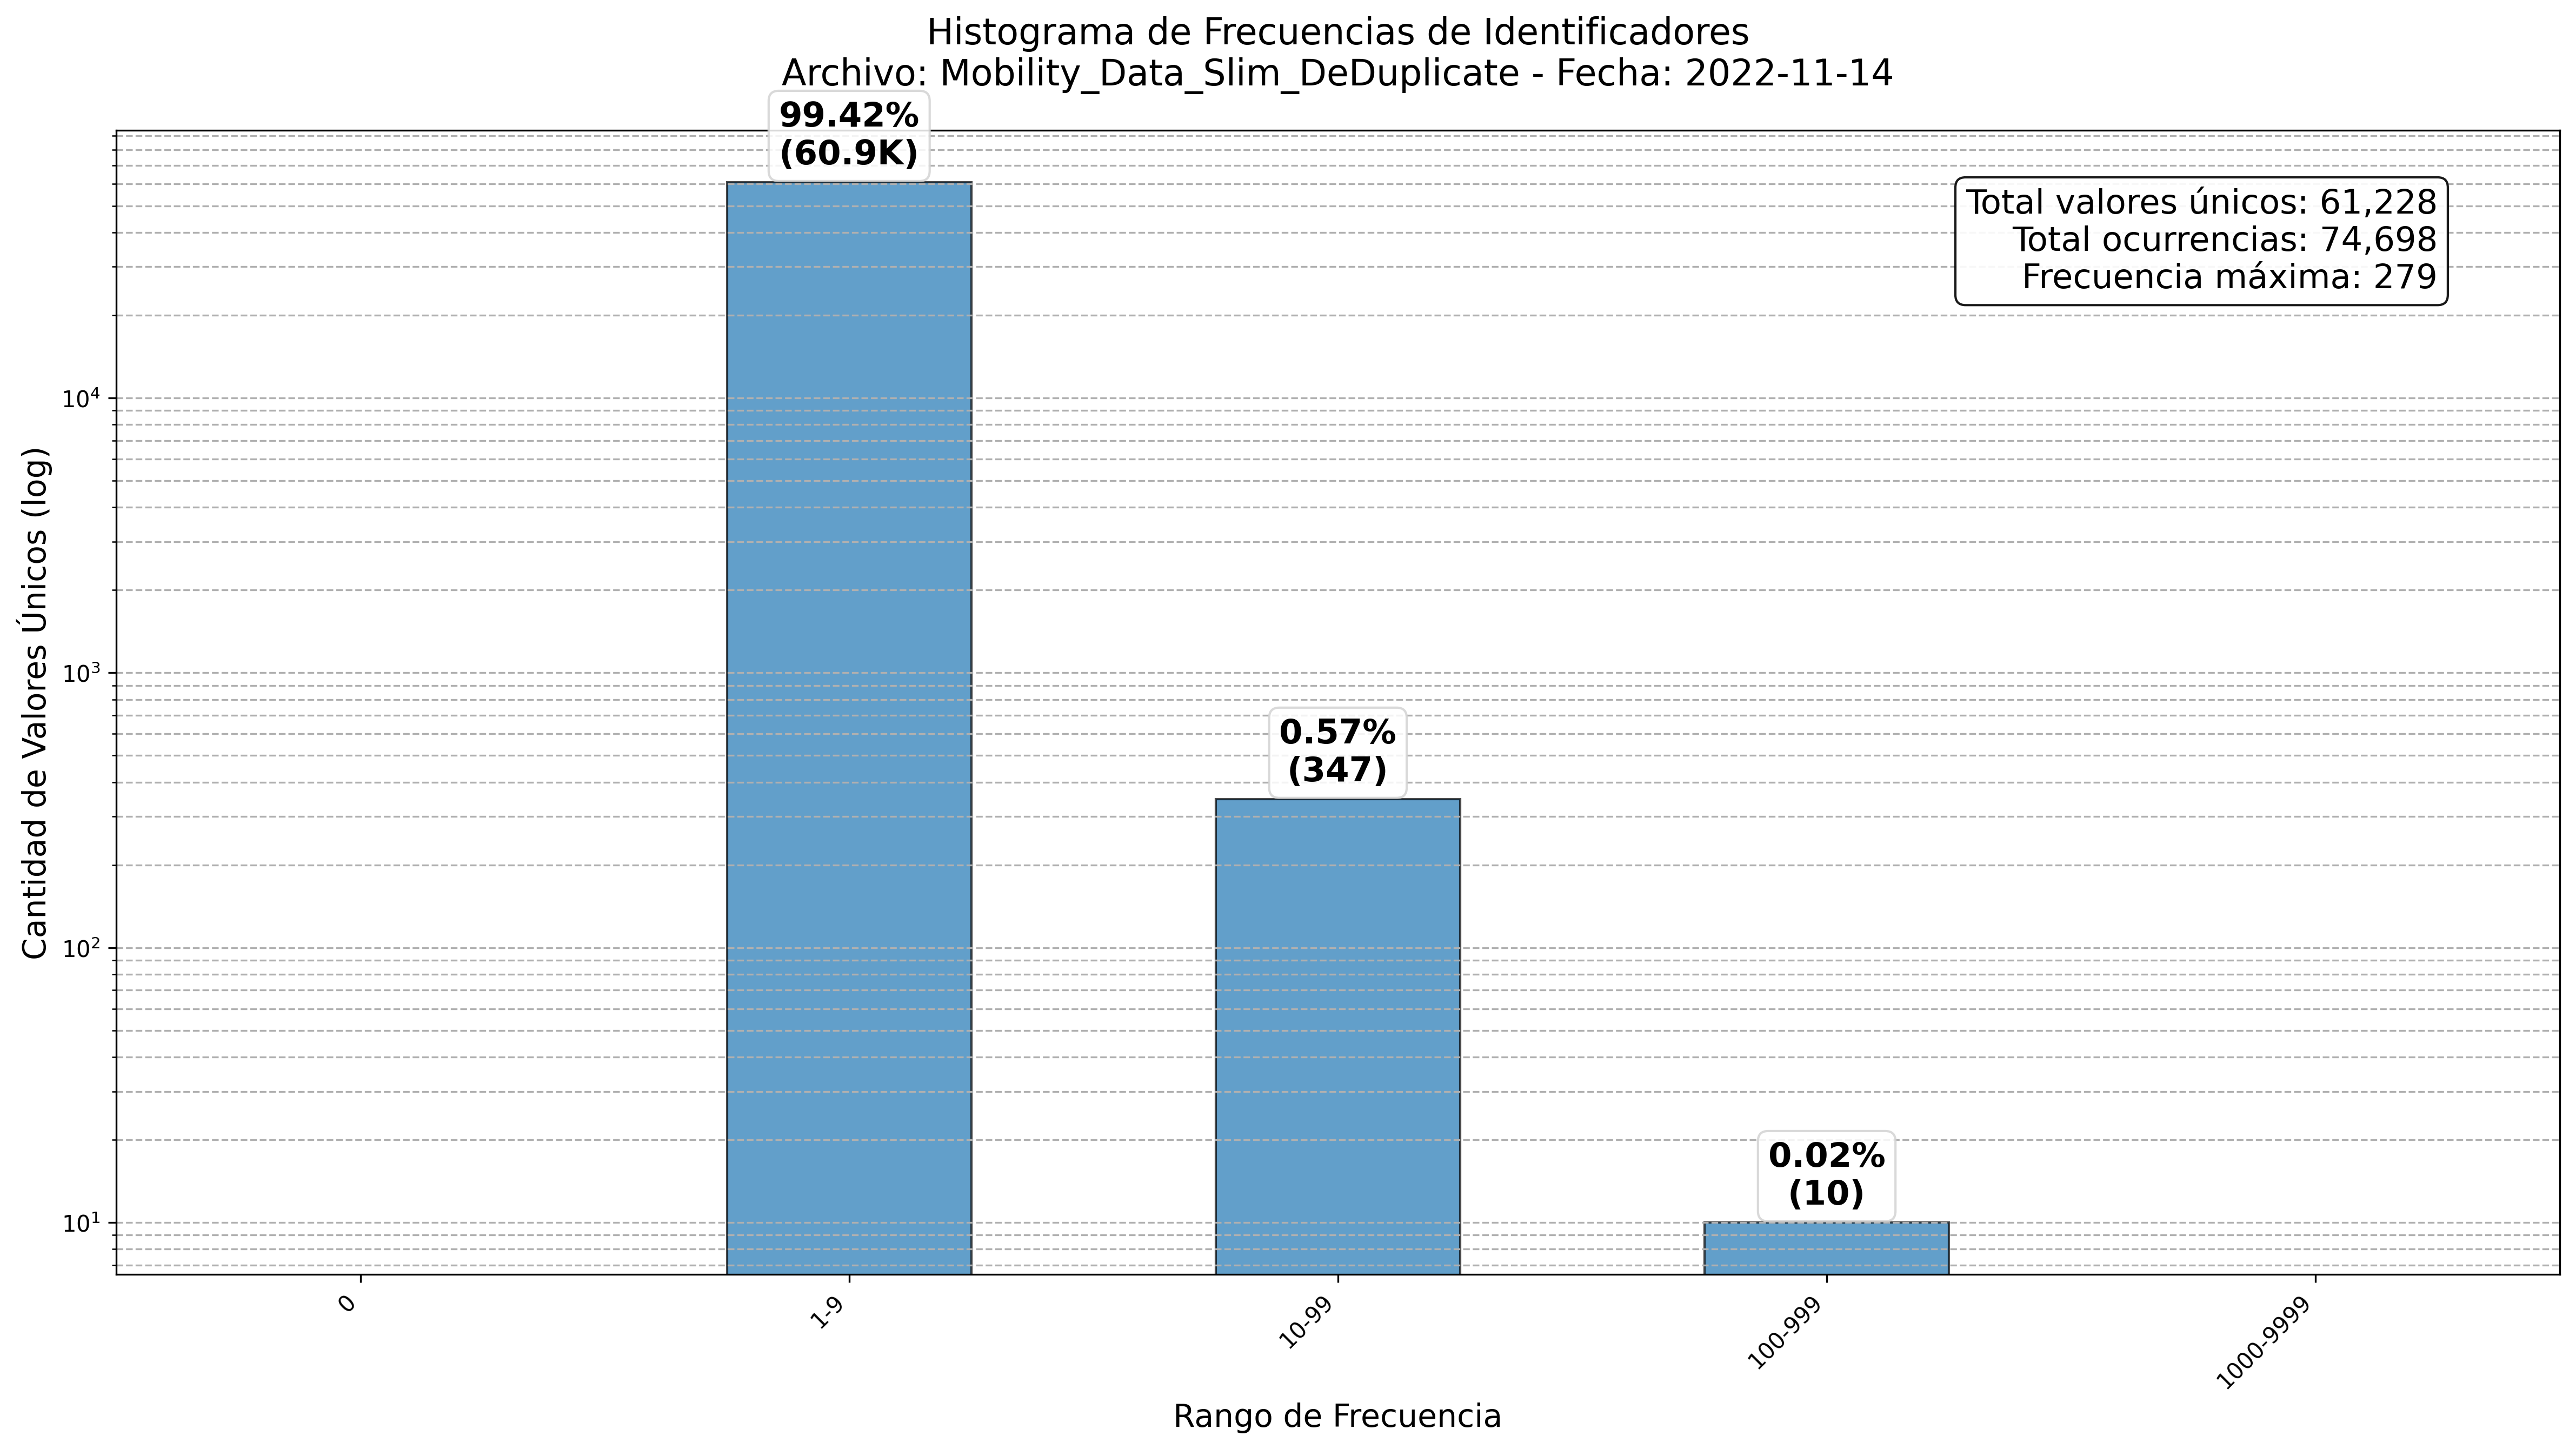
\includegraphics[width=\linewidth]{img/daily_histograms/histograma_identifier_Mobility_Data_Slim_DeDuplicate_2022-11-14.png}
        \caption{Histograma del 14/Nov/2022}
        \label{fig:sub9}
    \end{subfigure}
    \hfill
    \begin{subfigure}[t]{0.48\textwidth-1em}
        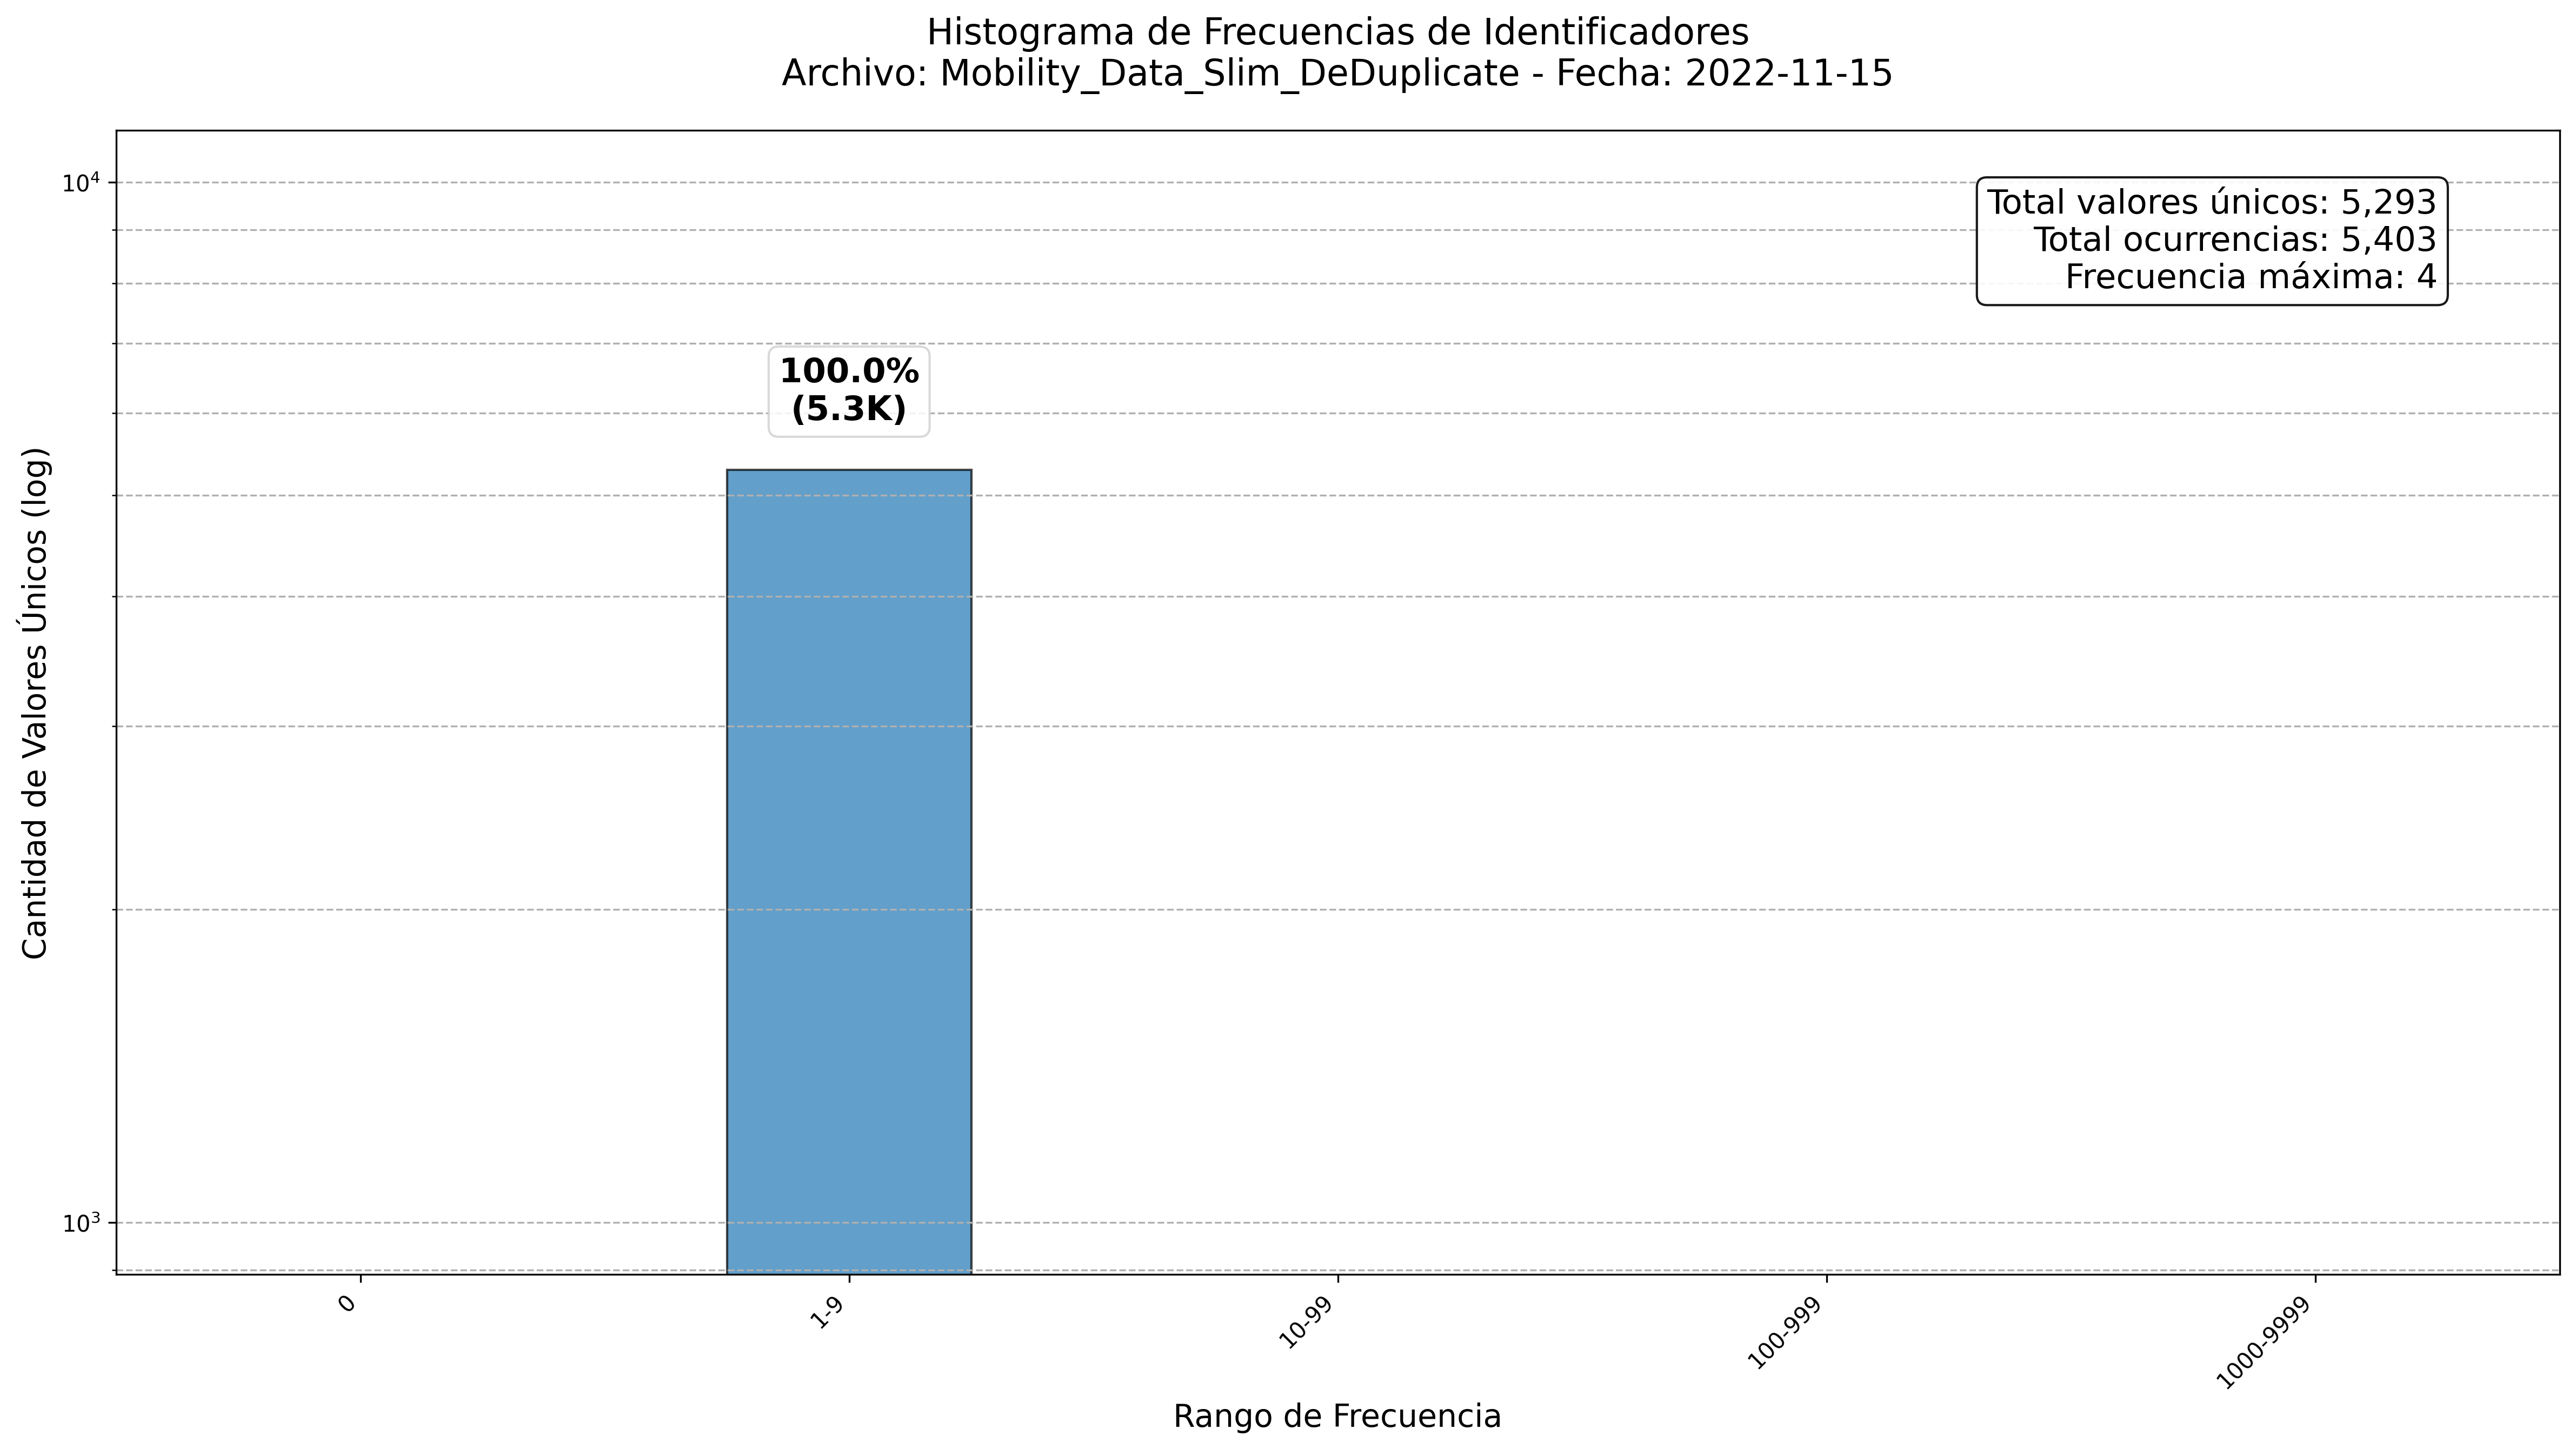
\includegraphics[width=\linewidth]{img/daily_histograms/histograma_identifier_Mobility_Data_Slim_DeDuplicate_2022-11-15.png}
        \caption{Histograma del 15/Nov/2022}
        \label{fig:sub10}
    \end{subfigure}
    \caption{Comparación de distribución de individuos por día.}
    \label{fig:histogramas_daily}
\end{figure}

De la figura anterior se puede observar que la distribución de individuos por día es bastante similar a la distribución vista en la Figura \ref{fig:identifier_histogram_deduplicate}, donde se observa que la mayoría de los individuos tienen una frecuncia de aparición baja. Además se puede ver que los primros seis días hay en promedio \textbf{1,400,000} de individuos, mientras que los últimos cuatro días este valor va disminuyendo hasta llegar a \textbf{5,293} individuos el día 15 de noviembre. Esto puede ser un indicativo de que la recolección de datos no fue constante a lo largo del tiempo, lo que podría deberse a diversos factores como problemas técnicos o cambios en el comportamiento de los individuos.

Un patrón que puede dar mucha información es determinar cuantos individuos tienen puntos de recorrido en más de un día. Para esto se ejecuta el código del Apéndice 

\begin{figure}[H]
  \centering
  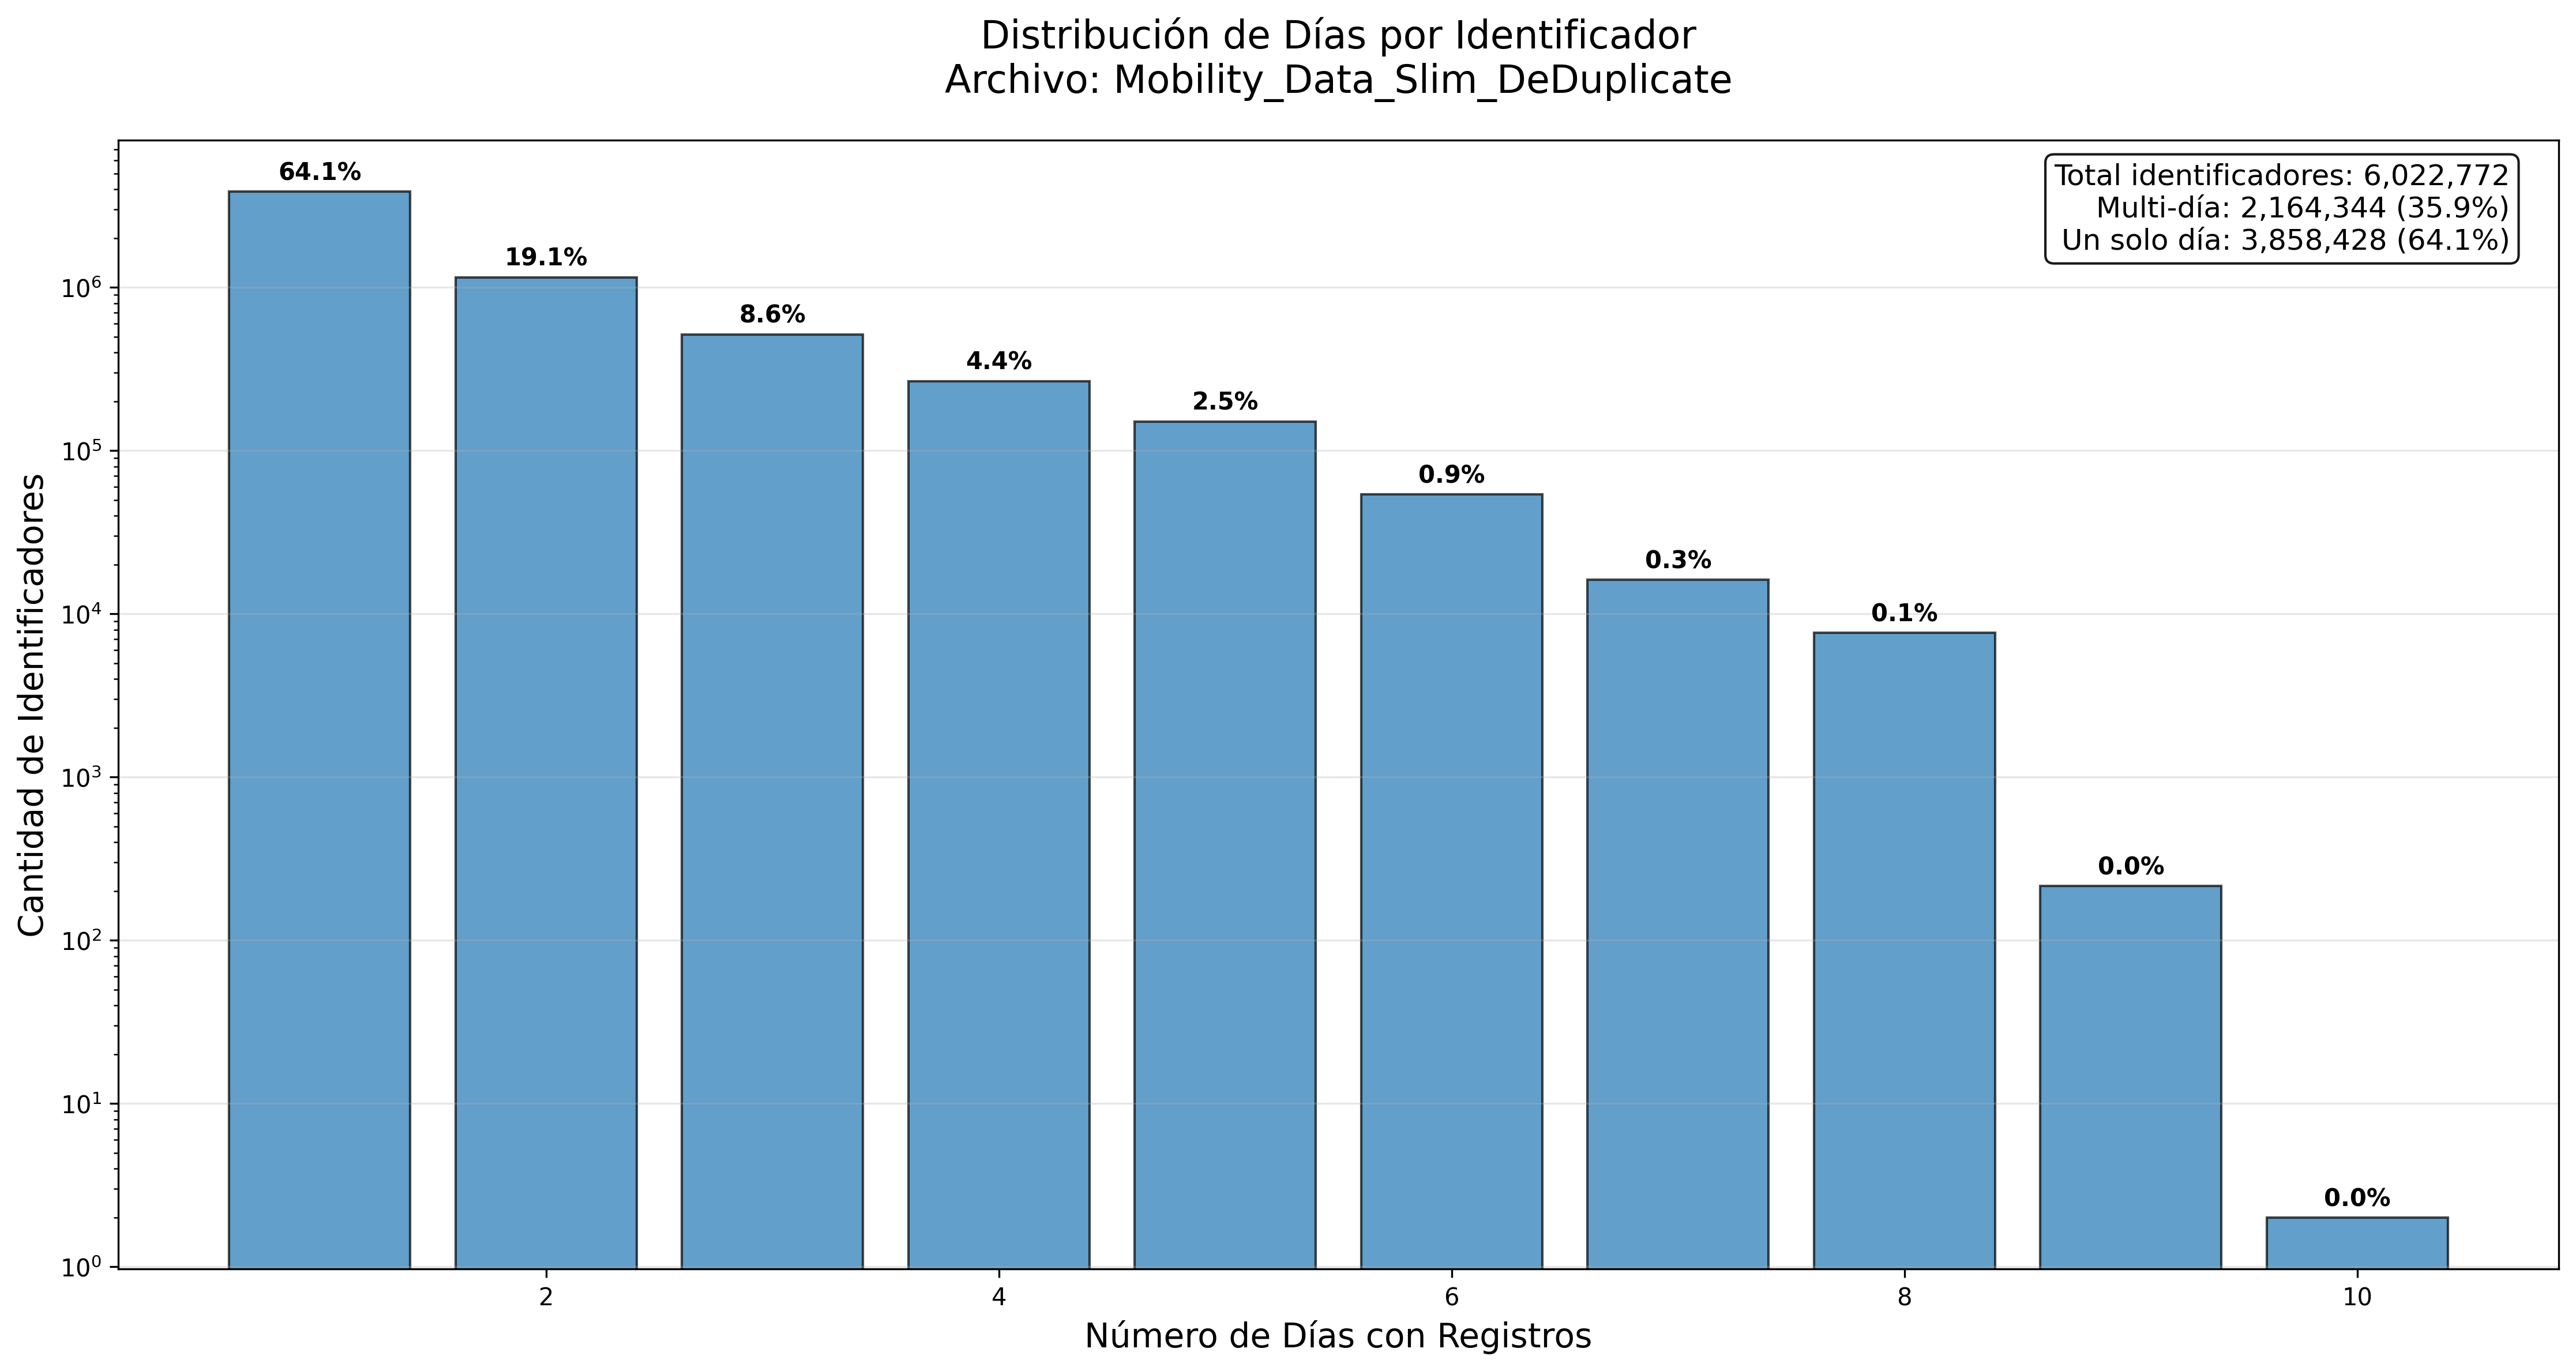
\includegraphics[width=\textwidth]{img/multi_day_analysis_Mobility_Data_Slim_DeDuplicate.png}
  \caption{Distribución de individuos por días.}
  \label{fig:multi_day_analysis}
\end{figure}

El resultado de este análisis se muestra en la figura anterior, donde se puede observar que el \textbf{64.06\%} de los individuos tienen puntos de recorrido en un día nada más, esto representa \textbf{3,858,428} individuos. Por otro lado, el porcentaje de individuos que tienen puntos de recorrido en más de seis días es del \textbf{0.4\%}, lo que representa \textbf{77,878} individuos. Este análisis es importante porque permite identificar a los individuos que tienen un comportamiento más rutinario y que podrían ser más relevantes para el estudio de patrones de movilidad. 

Con esta información se puede realizar un análisis más detallado de las trauectorias de los individuos del conjunto de datos. Por ejemplo, se puede identificar a los individuos que tienen puntos de recorrido en más de un día y que además tienen una alta frecuencia de aparición en esos días. Para esto se puede utilizar un gestor de base de datos como PostgreSQL, que permite realizar consultas complejas y obtener información más detallada sobre los individuos y sus trayectorias.

Para lograr esto, se puede utilizar el servicio de PostgreSQL creado al levantar el contenedor de Docker, como se describe en el Apéndice \ref{cod:docker_compose_file}. Es necesario crear una base de datos y una tabla para almacenar los datos. Importar los datos del archivo CSV a esta tabla se hace mediante el código del Apéndice \ref{cod:migrate_csv_to_postgres}. Una vez que los datos están en la base de datos, se pueden realizar consultas para obtener información más detallada sobre los individuos y sus trayectorias. A continuación, se exploraran algunos queries que permiten obtener información relevante sobre los individuos y sus trayectorias.

